\documentclass{article}
\usepackage[utf8]{inputenc}

\usepackage[italian]{babel}

\usepackage{tabularx}
\usepackage{natbib}
%\usepackage[demo]{graphicx}
\usepackage{graphicx}

%\usepackage[margin=1.0in]{geometry}

\usepackage{hyperref} %per i link
\usepackage{tikz}
\usepackage{comment}
\usepackage{subfigure}
\usepackage{subcaption}
\usepackage{caption}
\usepackage{subfloat}
\usepackage{amsmath, amsthm}

\usepackage{mathrsfs}

\usepackage{pgfplots}
\pgfplotsset{compat=1.18}
\usepackage{caption}

\theoremstyle{definition}
\newtheorem{rich}{richiamo matematico}[section]


%roba che crea comando per centrare immagine dentro immagine piu grande
%https://tex.stackexchange.com/a/308286
\newlength{\imagew}
\newlength{\imageh}
\newlength{\legendw}
\newlength{\legendh}
\newlength{\legendx}
\newlength{\legendy}
\newcommand{\graphicswithlegend}[6]{
	\setlength{\imagew}{#1}
	\settoheight{\imageh}{\includegraphics[width=\imagew]{#2}}
	
	\setlength{\legendw}{#3\imagew}
	\settoheight{\legendh}{\includegraphics[width=\legendw]{#4}}
	
	\setlength{\legendx}{\imagew}
	\addtolength{\legendx}{-\legendw}
	\addtolength{\legendx}{-#5\imagew}
	
	\setlength{\legendy}{\imageh}
	\addtolength{\legendy}{-\legendh}
	\addtolength{\legendy}{-#6\imageh}
	
	\includegraphics[width=\imagew]{#2}%
	\llap{
		\hspace{-\the\legendx}
		\raisebox{\legendy}{\includegraphics[width=\legendw]{#4}}
		\hspace{\the\legendx}
	}
}

\title{Circuiti 3}
\author{Diana Broggi, Giulia Cantarini, Paolo Falconelli}
\date{Laboratorio di fisica II}

\begin{document}

\maketitle
\tableofcontents
\section{Introduzione}
L'esperienza è volta allo studio delle funzioni di trasferimento\footnote{funzione che caratterizza il comportamento di un qualsiasi sistema dinamico mettendo in relazione ingresso e uscita} relative ai circuiti RC, RL ed RCL. \\\\
In un circuito lineare\footnote{circuito costituito solo da componenti la cui relazione costitutiva, algebrica o differenziale, è lineare} una funzione di trasferimento si definisce in relazione a due nodi, come il rapporto tra il segnale (nel nostro caso una tensione) nel nodo di uscita e il segnale dal nodo di ingresso. In generale essa dipende dalla frequenza del segnale di riferimento, perciò in laboratorio è stato adoperato il generatore di funzioni con un segnale di tipo sinusoidale a frequenza modificabile; per esprimere gli effetti del circuito sia sull'ampiezza che sulla fase del segnale trasferito, la funzione di trasferimento è una funzione a valori complessi. \\
\[\vec{H}(\omega)= \frac{\vec{V}_{in}(\omega)}{\vec{V}_{out}(\omega)}\]

dove \(\vec{V}_{in}\) e \(\vec{V}_{out}\) sono fasori\footnote{vettori nel piano complesso utilizzati in elettrotecnica come notazione privilegiata per rappresentare un segnale sinusoidale. Es: \(V(t) = Asin(\omega t + \phi )\)} che descrivono il segnale variabile con \(\omega\) in ingresso e in uscita. 
\section{Strumentazione}
La strumentazione adoperata per la realizzazione dei circuiti e la raccolta dati comprende:
\begin{itemize}
    \item generatore di funzioni d'onda, utilizzato per produrre un segnale a tensione alternata di \(V_{pp} = 20\)V; resistenza interna di \(671 \pm 1 \Omega\).
    \item oscilloscopio, permette di visualizzare l'andamento temporale del segnale ricevuto dalle sonde, e di effettuare le  misure necessarie del caso attraverso la funzione \textit{Acquire}; reistenza interna \(\approx\) 1 \(M\Omega\) e capacità di ingresso di 20pF.
    \item cavi coassiali, utilizzati per trasmettere il segnale dal generatore all'oscilloscopio; reistenza dell'ordine dei 50\(\Omega\).
    \item sonde compensate a 10x, adoperate per misurare la tensione in determinati nodi del circuito e riferirla in ingresso all'oscilloscopio.
    \item \textit{breadboard}.
    \item resistenze dell'ordine dei \(k\Omega\).
    \item condensatori con capacità  dell'ordine dei nF.
    \item induttori di induttanza che varia dell'ordine dei mH ad H.
  
\end{itemize}

\label{sec:PrimaParte}
\section{Parte prima}
Nella prima parte dell'esperienza abbiamo analizzato il trasferimento del segnale alternato attraverso i circuiti RC ed RL. Si osserva che in regimi di corrente alternata, ad elementi circuitali quali C ed L è associata una reattanza X dovuta all'opposizione di tali elementi alla variazione di corrente nel circuito. In tali condizioni la legge di Ohm risulta estesa a V = \(I \cdot Z\) dove Z è il numero complesso \(Z :=  R + jX\) detto induttanza e tiene conto di entrambi i fenomeni di opposizione di un circuito al passaggio di corrente alternata: fenomeni di consumo di energia elettrica (passaggio attraverso R) e fenomeni di accumulo di energia elettromagnetica (passaggio per X). \\
Il calcolo delle induttanze si esegue a partire dalla relazione costitutiva dei relativi elementi
\begin{enumerate}
    \item[-] impedenza capacitiva \(Z_{C}\) \\
   da \(I = C \dot{V}\), pondendo \(V = V_{0}e^{j\omega t }\) e \(I = I_{0}e^{j(\omega t + \phi)}\), otteniamo: \[ I_{0}e^{j(\omega t + \phi)} = C j\omega V_{0}e^{j\omega t } \rightarrow \frac{V}{I} = \frac{1}{Cj\omega} = Z_{C}\]
   
    \item[-] impedenza induttiva \(Z_{L}\) \\
   da \(V = L \dot{I}\), pondendo \(V = V_{0}e^{j(\omega t + \phi)}\) e \(I = I_{0}e^{j(\omega t + \phi)}\), otteniamo: \[ V_{0}e^{j(\omega t + \phi)} = L j\omega V_{0}e^{j\omega t } \rightarrow \frac{V}{I} = Lj\omega = Z_{L}\]
   
    \item[-] impedenza resistiva \(Z_{R}\) \\
    da \(V = I R\) risulta facilmente \(\frac{V}{I} = R = Z_{R}\)
\end{enumerate}
\subsection{Procedimento adottato}
La rappresentazione di \(\vec{H}\) in funzione di f richiede di realizzare due grafici: uno per il modulo ed uno per la fase; il modulo di H si ottiene tramite il rapporto dei moduli di \(\vec{V}_{out}\) e \(\vec{V}_{in}\) mentre la fase è pari alla differenza delle fasi. Tali misure sono state ottenute tramite la funzione \textit{Acquire} dell'oscilloscopio selezionando ampiezza e sfasamento rispetto al segnale di entrata. \\
I circuiti interessati per questa prima parte corrispondono allo schema in Figura \ref{fig:schemaZR} in cui si può sostituire Z con C od L a seconda del caso in esame. \\

\noindent Grazie alla funzione \textit{Math} dell'oscilloscopio abbiamo potuto osservare contemporaneamente sullo schermo i segnali rilevati in corrispondenza delle sonde e la loro differenza. Questa operazione permette di misurare nello stesso momento il potenziale in uscita ai capi di R e quello ai capi di Z senza dover invertire i due componenti, permette quindi di risparmiare del tempo. \\ 
Le misure per \(V_{A}\), \(V_{B}\) e \(V_{AB}\), che corrispondono rispettivamente alle ampiezze picco-picco di \(\vec{V}_{in}\), \(\vec{V}_{out}\) ai capi di R e \(\vec{V}_{out}\) ai capi di Z, sono stati raccolti in tabella assieme alle relative fasi (che fanno riferimento a \(\vec{V}_{in}\)) \(\phi_{B}\) e \(\phi_{AB}\). Abbiamo infine eseguito il fit per ogni grafico di  \(\left|H\right|\) e \(\phi_{H}\) attraverso il software ROOT di CERN dopo aver ricavato l'andamento atteso secondo la teoria.  

\begin{figure}[!ht]

	\makebox[1 \textwidth][c]{       %centering table
		\resizebox{0.50 \textwidth}{!}{   %resize table
			\includegraphics{RZschema.png}
		} %close resize
	} %close centering
	\caption{schema di un circuito ZR generico}

    \label{fig:schemaZR}

\end{figure}
\subsection{Circuito RC}
\subsubsection{Funzione di trasferimento su C}
Per ricavare \(\vec{H}\) su C dalla teoria sui circuiti in corrente alternata, è necessario conoscere l'andamento del potenziale ai capi di C, perciò applichiamo l'estensione della legge di Ohm come segue
\[\vec{V_{C}}(t) = \vec{I}(t) \cdot Z_{C} =  \frac{\vec{V_{g}}}{1 + j \omega R C }\]

\noindent dove il simbolo di vettore su \(V_{C}\) ed I sta ad indicare semplicemente che si tratta di segnali sinusoidali, si ricorda che anche Z è un elemento del campo complesso quindi in caso di necessità può essere visto anche come vettore. 

\noindent Siccome \(\vec{H}= \frac{\vec{V_{C}}(t)}{\vec{V_{g}}(t)}\), la rappresentazione di H come elemento dello spazio vettoriale complesso è

\[\vec{H} =  \frac{1}{1 + j \omega R C }\]

\noindent riconosciamo infine modulo e fase nelle seguenti espressioni
\[\left| \vec{H} \right| = \frac{1}{\sqrt{1 +  \omega^2 R^2 C^2}} \hspace{1cm} \phi_{\vec{H}} = 0 - arctan(R \omega C)\]

\noindent le quali sono state considerate come modello funzionale per eseguire l'interpolazione dei punti ottenuti dalla raccolta dati. 

\subsubsection*{Dati raccolti}
Utilizzando l'oscilloscopio, abbiamo potuto visualizzare i segnali sinusoidali di \(\vec{V}_{in}(t)\), \(\vec{V}_{out}(t)\) ai capi di C e \(\vec{V}_{out}(t)\) ai capi di R. \\
La raccolta dati è stata svolta registrando le misure ottenute per le relative ampiezze picco-picco e fasi dopo aver selezionato la funzione \textit{Acquire} dell'oscilloscopio; per ogni misura abbiamo raccolto un solo valore in quanto era l'unico ad essere rappresentato sullo schermo, tuttavia associamo a tali letture un errore strumentale dell'1\% (dedotto in base al numero di cifre significative rappresentate dallo strumento). \\
Osservando spesso dei punti interrogativi associati alle misure per \(\phi\), abbiamo ritenuto ragionevole attribuire un errore casuale del 2\% almeno ai valori più piccoli (inferiori a 10\(^{\circ}\)), quelli per cui un errore dell'1\% risulta piuttosto riduttivo rispetto ai limiti di costruzione dello strumento che riteniamo non trascurabili in questi casi. \\
L'errore associato al rapporto tra \(V_{A}\) e \(V_{AB}\), è dato dalla propagazione degli errori tramite la formula:

\[ \sigma_{\frac{V_{AB}}{V_{A}}} = \sqrt{ \left(\sigma_{VA} \cdot \frac{V_{AB}}{V_{A}^{2}}\right)^{2} + \left(\frac{\sigma_{V_{AB}}}{V_{A}}\right)^{2} }\]

\noindent La seguente tabella racchiude solo i dati necessari all'analisi del potenziale ai capi di C, si noti che sia \(V_{A}\) che \(V_{AB}\) sono le ampiezze picco-picco delle relative funzioni sinusoidali. 
\begin{table}[!htbp]
\centering
    \captionsetup{labelformat=empty}
    	 \caption{RC - misure ai capi di C}
    \resizebox{12.2cm}{!}{

    \begin{tabular}{c|c|c|c|c}

        frequenza[Hz] & \(V_{A}\)[V] & \(V_{AB}\)[V] & \(V_{AB}/V_{A}\) & \(\phi_{AB}\) \\
        \hline
        \hline
        1       & 16.4$\pm$0.2         & 16.4$\pm$0.2         & 1.00 $\pm$ 0.01 & -0.72 $ \pm$ 0.02\\
        10      & 20.3$\pm$0.2         & 20.3 $\pm$ 0.2         & 1.00 $\pm$ 0.01 & -3.24 $\pm $ 0.09\\
        50      & 20.1$\pm$0.2         & 19.2$\pm$0.2   & 0.96 $\pm$ 0.01 & -15.6 $\pm $ 0.2\\
        100     & 20.6$\pm$0.2      & 17.6$\pm$0.2         & 0.85 $\pm$ 0.01 & -31.2 $ \pm$ 0.4\\
        120     & 20.2$\pm$0.2        & 16.4$ \pm$0.2         & 0.81 $\pm$ 0.01 & -34.5 $ \pm$ 0.5\\
        150     & 20.2$\pm$0.2         & 15.0$ \pm$0.2    & 0.74 $\pm$ 0.01 & -40.5 $ \pm$ 0.6\\
        163     & 20.2$\pm$0.2       & 14.6$\pm$0.1     & 0.72 $\pm$ 0.01 & -43.5 $\pm $ 0.6\\
        170     & 20.2$\pm$0.2         & 14.4$\pm$0.1   & 0.71 $\pm$ 0.01 & -45.0 $\pm $ 0.6\\
        200     & 20.0$\pm$0.2& 13.1$\pm$0.1         & 0.655 $\pm$ 0.009 & -50.1 $\pm $ 0.7\\
        400     & 20.0$\pm$0.2             & 7.82$\pm$0.08        & 0.391 $\pm$ 0.006 & -66.2 $\pm $ 0.9\\
        600     & 20.0$\pm$0.2            & 5.40$\pm$0.05  & 0.270 $\pm$ 0.004 & -74 $\pm $ 1\\
        800     & 19.9$\pm$0.2         & 4.04$\pm$0.04        & 0.203 $\pm$ 0.003 & -78 $\pm $ 1\\
        900     & 19.9$\pm$0.2         & 3.60$\pm$0.04  & 0.181 $\pm$ 0.003 & -79 $\pm $ 1\\
        950     & 19.9$\pm$0.2         & 3.44$\pm$0.03        & 0.173 $\pm$ 0.002 & -80 $ \pm$ 1\\
        1000    & 19.9$\pm$0.2         & 3.20$\pm$0.03  & 0.161 $\pm$ 0.002 & -80 $\pm $ 1\\
        1050    & 19.9$\pm$0.2         & 3.12$\pm$0.03        & 0.157 $\pm$ 0.002 & -81 $ \pm$ 1\\
        1100    & 19.9$\pm$0.2         & 2.96$\pm$0.03        & 0.149 $\pm$ 0.002 & -81 $ \pm$ 1\\
        1200    & 19.9$\pm$0.2         & 2.64$\pm$0.03        & 0.133 $\pm$ 0.002 & -82 $\pm $ 1\\
        1400    & 19.9$\pm$0.2         & 2.32$\pm$0.02        & 0.117 $\pm$ 0.002 & -83 $\pm $ 1\\
        1600    & 19.9$\pm$0.2         & 2.00$\pm$0.02     & 0.101 $\pm$ 0.001 & -84 $\pm $ 1\\
        2000    & 20.0$\pm$0.2     & 1.80$\pm$0.02  & 0.090 $\pm$ 0.001 & -85 $ \pm$ 1\\

        \hline
        \hline
    \end{tabular}
    }
\caption{errore strumentale: 1\%}
\end{table}

\subsubsection*{Analisi dati}
Per osservare l'andamento del modulo abbiamo costruito i grafici dei punti ottenuti considerando \(\frac{V_{AB}}{ V_{A}}\) in funzione della frequenza, mentre per la fase è bastato rappresentare \(\phi_{AB}\) in funzione della frequenza; abbiamo poi eseguito le due interpolazioni per i modelli attesi, sostituendo a \(\omega = 2\pi f = 2 \pi x\), ottendendo così:

\begin{figure}[!h]
\caption{RC - funzione di trasferimento ai capi di C}

    \makebox[1 \textwidth][c]{       %centering table
		\resizebox{1.20 \textwidth}{!}{   %resize table
\hfill
\subfigure[modulo]{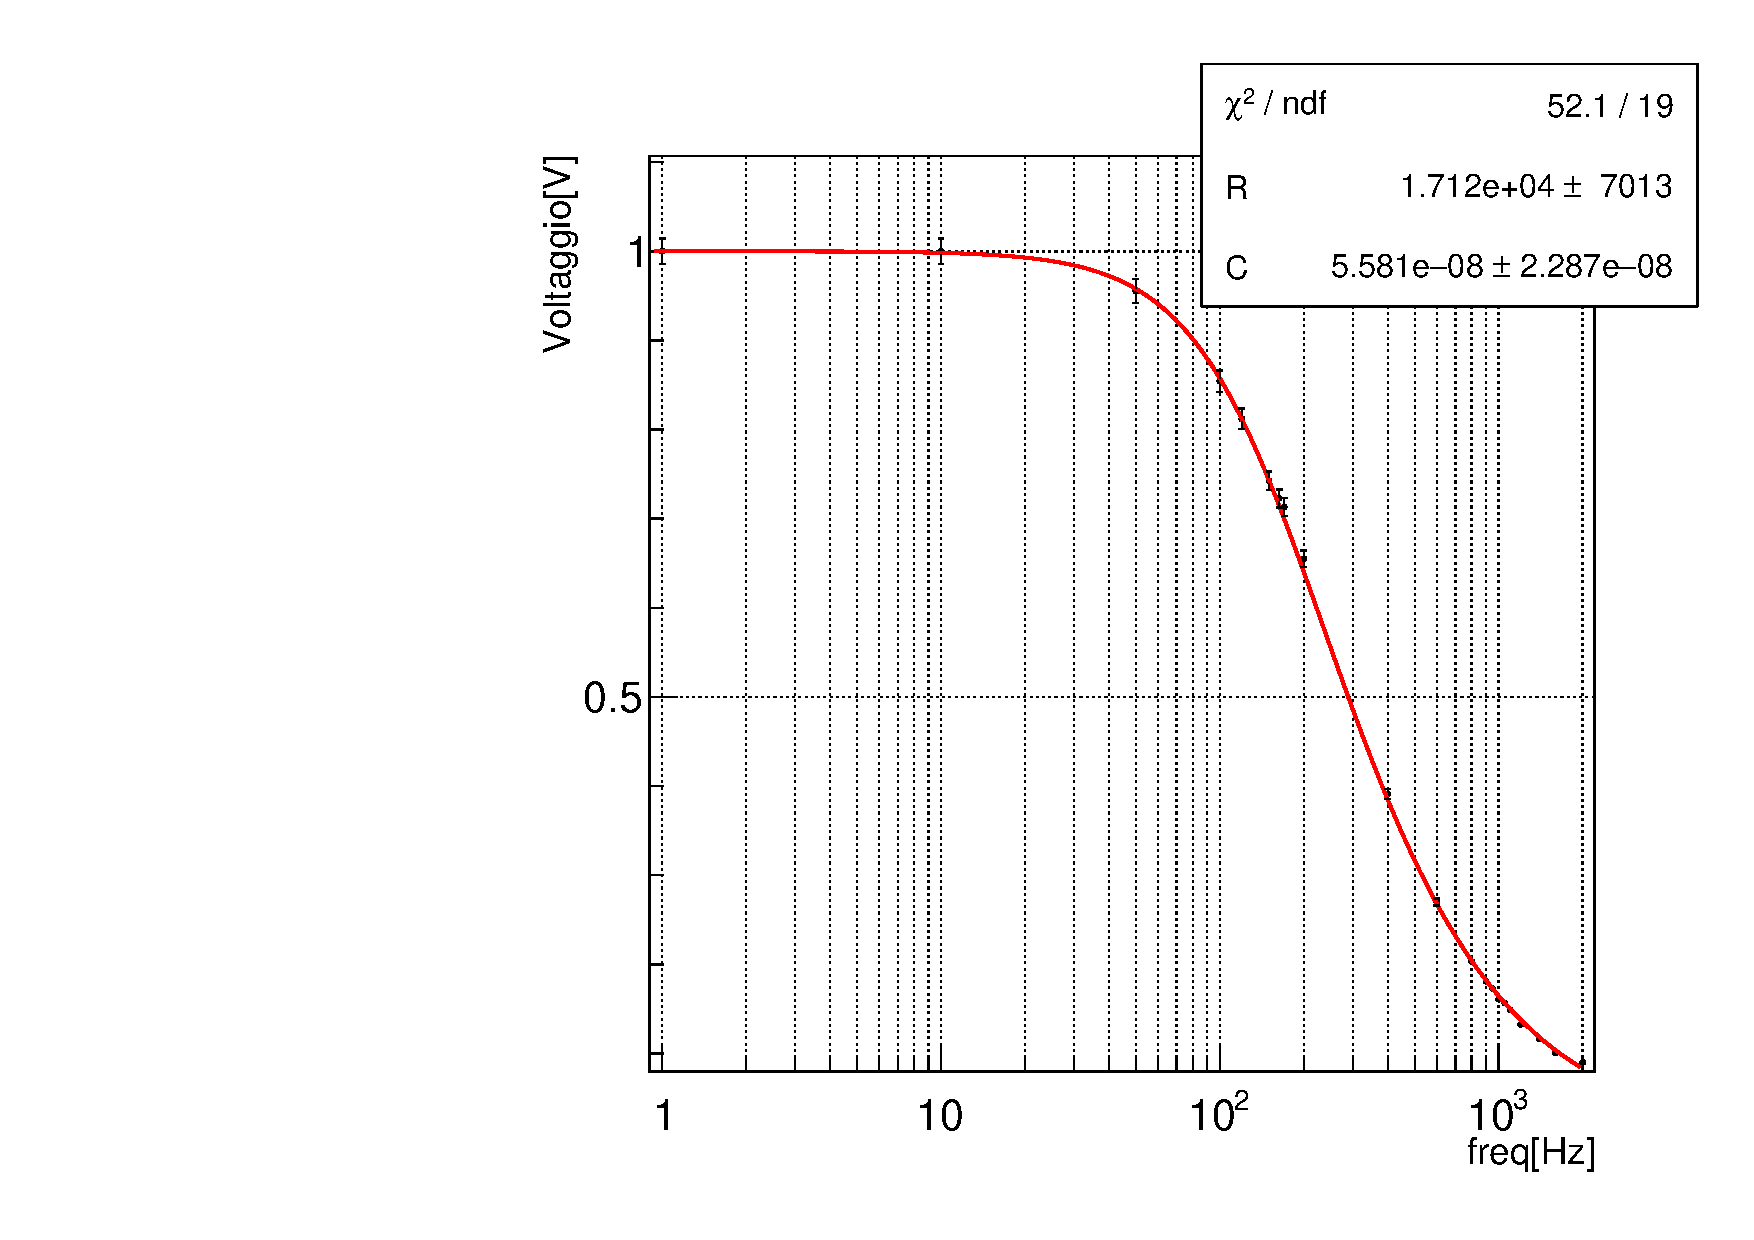
\includegraphics[width=5.7cm]{RC/RC-modulo-capoC.pdf}}
\hfill
\subfigure[fase]{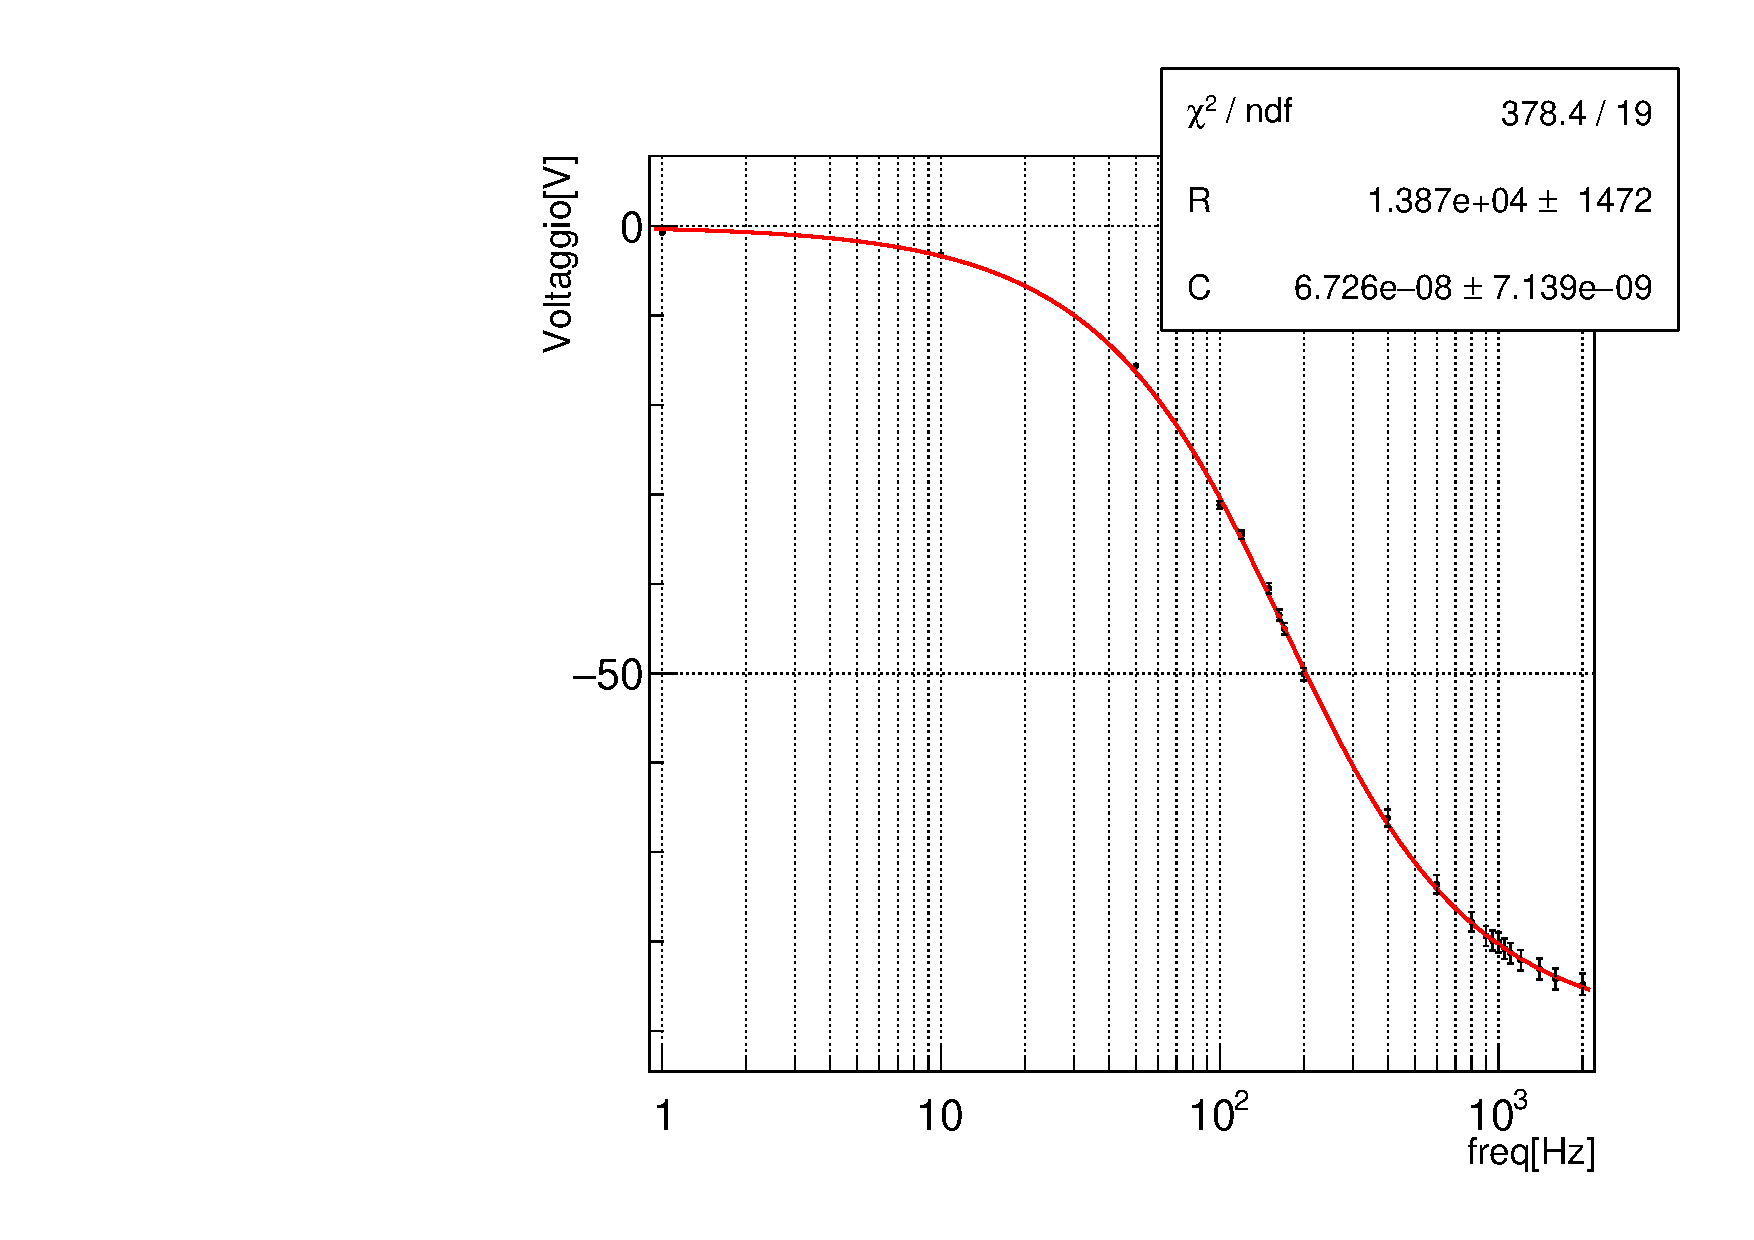
\includegraphics[width=5.7cm]{RC/RC-fase-capoC.pdf}}
\hfill
    }
}
\caption*{dal grafico in figura (a) si può riconoscere il ruolo di filtro passa basso ricoperto dalla capacità in un circuito RC, siccome per frequenze piccole \(\frac{V_{AB}}{V_{A}} \approx 1\) }
\label{fig:RC_su_C}
\end{figure}

\noindent Il test del chi quadro effettuato per constatare il livello di compatibilità dei dati con il modello atteso non è soddisfatto in maniera accettabile in nessuno dei due casi; dobbiamo questo insuccesso non tanto ad un errore sistematico nella determinazione del modello (i punti si dispongono come previsto attorno alla curva) quanto nella stima degli errori casuali, che riteniamo sottostimati in quanto \(\frac{\chi^{2}}{Ndf} > 1\) per entrambi i test. \\\\
Per quanto riguarda il modulo di H, possiamo supporre la presenza di un errore casuale dovuto al fatto che \(V_{AB}\) è il modulo di una funzione sinusoidale risultata dalla differenza (eseguita con \textit{Math}) tra \(\vec{V}_{out}\) e \(\vec{V}_{in}\), due segnali sinusoidali affetti da rumore elettronico. Nonostante in laboratorio si sia fatto uso della funzione \(\textit{Get Mean}\) per ottenere un valore medio del segnale desiderato al fine di ridurre il rumore, questo non può essere ridotto a zero, perciò riconosciamo un \(\sigma_{noise} \neq 0\) da associare a \(\vec{V}_{out}\) e \(\vec{V}_{in}\) e supponiamo che questo si propaghi sulla loro differenza moltiplicato per \(\sqrt{2} \rightarrow \sigma_{V_{out} - V_{in}} = \sqrt{2}\cdot \sigma_{noise}\). Dunque risulta che \(V_{AB}\), ampiezza picco-picco di \(\vec{V}_{out} - \vec{V}_{in}\), essendo la distanza tra un picco ed un ventre della funzione, viene intaccata da un errore casuale pari a \(\sqrt{2} \cdot \sqrt{2} \cdot \sigma_{noise}\); mentre l'ampiezza picco-picco \(V_{A}\) viene intaccata da un errore \(\sqrt{2} \cdot \sigma_{noise}\). \\ I due errori si sommano come riportato nella formula di propagazione nel paragrafo precedente.\\\\
Per quanto riguarda la fase di H rispetto al segnale in entrata, il suo errore casuale dipende da \(\sigma_{t}\) (infatti \(\Delta \phi = \Delta t \omega\)), il quale risente dell'incertezza su V secondo: \( \sigma_{t} = \frac{\sigma_{V}}{\frac{dV}{dt}} = \frac{\sqrt{2} \cdot \sigma_{noise}}{\frac{dV}{dt}}\); questo potrebbe spiegare, supponendo un rumore sufficiente, anche l'insuccesso del test per il secondo grafico. \\

\noindent La sorgente più comune di rumore negli apparati elettronici è il rumore termico, intrinseco di ogni elemento dissipativo. \\

\noindent Osserviamo i risultati numerici ricavati da queste due interpolazioni:
\begin{enumerate}
    \item[-] C dall'interpolazione per il modulo: \(C_{1} = 5.581 \cdot 10^{-8} \pm 2.287 \cdot 10^{-8}\) F
    \item[-] C dall'interpolazione per la fase: \(C_{2} = 6.726 \cdot 10^{-8} \pm 0.713 \cdot 10^{-8} \)F
\end{enumerate}
poste a confronto con il test t-Student danno una probabilità di compatibilità del 61.7\%:
\[t = \frac{\left| C_{1} - C_{2} \right|}{\sqrt{\sigma^{2}_{C1} + \sigma^{2}_{C2}}} = 0.5 \rightarrow PValue = 61.7\%\]

\noindent Sarà utile in seguito conoscere il valore medio di queste due stime, ricaviamo dunque \(C_{best}\) eseguendo la media pesata coi pesi = \(w_{i} = \frac{1}{\sigma^{2}_{i}}\):

\[C_{capoC} = \frac{\sum{C_{i} \cdot w_{i}}}{\sum{w_{i}}}\pm \frac{1}{\sqrt{\sum{w_{i}}}} = 6.625 \cdot 10^{-8} \pm 0.681 \cdot 10^{-8} F\]

\noindent Per completezza confrontiamo anche i valori ottenuti per R:
\begin{enumerate}
    \item[-] R ottenuto dall'interpolazione per il modulo: \(R_{1} = 17120 \pm 7013 \Omega \)
    \item[-] R ottenuto dall'interpolazione per la fase: \(R_{2} = 13870 \pm 1472 \Omega\)
\end{enumerate}

risulta un valore per t pari a 0.5 che corrisponde ancora una volta ad una probabilità che le due stime siano compatibili del 61.7\%. Abbiamo calcolato la media pesata tra le due stime per ottenere \(R_{capoC} =  14007 \pm  1441\Omega\).

\subsubsection{Funzione di trasferimento su R}
Applichiamo di nuovo la legge di Ohm, questa volta per ricavare \(\vec{V_{R}}\):
\[\vec{V}_{R}(t) = \vec{I}(t) \cdot R = \frac{\vec{V}_{g}(t) \cdot R}{R + \frac{1}{j\omega C}}\]

\[\Downarrow\]

\[\vec{H} = \frac{R}{R +\frac{1}{j\omega C}}\]
il modulo e la fase di H ai capi di R sono dunque:
\[\left| \vec{H} \right| = \frac{R \omega C}{\sqrt{1 + R^2 \omega^2 C^2}} \hspace{1cm} \phi_{\vec{H}} = \frac{\pi }{2} - arctan(R \omega C)\]


\subsubsection*{Dati raccolti}
La raccolta dati è stata effettuata in contemporanea a quella descritta nel paragrafo precedente, trattandosi dello stesso circuito. La valutazione di errori strumentali e casuali rimane dunque la medesima. Questa volta ci concentriamo però sui dati rilevati ai capi di R, dunque \(V_{B}\) e \(\phi_{B}\); ancora una volta l'errore associato al rapporto tra \(V_{A}\) e \(V_{B}\) è dato dalla propagazione degli errori:

\[ \sigma_{\frac{V_{B}}{V_{A}}} = \sqrt{ \left(\sigma_{VA} \cdot \frac{V_{B}}{V_{A}^{2}}\right)^{2} + \left(\frac{\sigma_{V_{B}}}{V_{A}}\right)^{2} }\]

\begin{table}[!htbp]
\centering
    \captionsetup{labelformat=empty}
    	 \caption{RC - misure ai capi di R}
    \resizebox{11.0cm}{!}{

    \begin{tabular}{c|c|c|c|c}
        frequenza[Hz] & \(V_{A}\)[V] & \(V_{B}\)[V] & \(V_{B}/V_{A}\) & \(\phi_{B}\)[gradi] \\
        \hline
        \hline
       1       & 16.4 $\pm $ 0.2      & 0.107 $\pm $ 0.001 & 0.00652 $ \pm$ 0.00009 & 92 $\pm $ 1\\
        10      & 20.3 $\pm $ 0.2    & 1.22 $\pm $ 0.01 & 0.0601 $\pm $ 0.0008 & 87 $\pm $ 1 \\
        50      & 20.1 $ \pm$ 0.2        & 5.84 $ \pm$ 0.06  & 0.291 $\pm $ 0.004 & 73 $\pm $ 1\\
        100     & 20.6 $\pm $ 0.2     & 10.4 $\pm $ 0.1  & 0.505 $\pm $ 0.007 & 58.0 $\pm $ 0.8\\
        120     & 20.2 $\pm $ 0.2       & 11.8 $\pm $ 0.1  & 0.584 $ \pm$ 0.008& 53.5 $\pm $ 0.8\\
        150     & 20.2 $\pm $ 0.2       & 13.4 $\pm $ 0.1 & 0.663 $\pm $ 0.009 & 48.1 $\pm $ 0.7\\
        163     & 20.2 $ \pm$ 0.2     & 14.1 $\pm $ 0.1 & 0.70 $\pm $ 0.01& 45.2 $\pm $ 0.6 \\
        170     & 20.2 $ \pm$ 0.2     & 14.4 $\pm $ 0.1& 0.71 $\pm $ 0.01 & 44.5 $\pm $ 0.6\\
        200     & 20.0 $\pm $ 0.2    & 15.5 $\pm $ 0.2    & 0.77 $\pm $ 0.01& 39.6 $\pm $ 0.6 \\
        400     & 20.0 $\pm $ 0.2    & 18.6 $\pm $ 0.2  & 0.93 $\pm $ 0.01& 21.9 $\pm $ 0.3  \\
        600     & 20.0 $\pm $ 0.2    & 19.2 $\pm $ 0.2  & 0.96 $\pm $ 0.01 & 15.1 $ \pm$ 0.2\\
        800     & 19.9 $\pm $ 0.2      & 19.4 $ \pm$ 0.2& 0.97 $ \pm$ 0.01& 11.6 $\pm $ 0.2 \\
        900     & 19.9 $ \pm$ 0.2  & 19.5 $\pm $ 0.2  & 0.98 $\pm $ 0.01& 8.2 $\pm $ 0.2\\
        950     & 19.9 $\pm $ 0.2        & 19.5 $\pm $ 0.2        & 0.98 $\pm $ 0.01    & 9.9 $\pm $ 0.3 \\
        1000    & 19.9 $\pm $ 0.2       & 19.5 $\pm $ 0.2       & 0.98 $\pm $ 0.01& 9.2 $\pm $ 0.3  \\
        1050    & 19.9 $ \pm$ 0.2       & 19.5 $\pm $ 0.2        & 0.98 $\pm $ 0.01& 8.8 $ \pm$ 0.2\\
        1100    & 19.9 $\pm $ 0.2 & 19.6 $\pm $ 0.2     & 0.98$\pm $ 0.01 & 7.9 $\pm $ 0.2\\
        1200    & 19.9 $\pm $ 0.2& 19.6 $\pm $ 0.2   & 0.98 $\pm $ 0.01& 7.3 $\pm $ 0.2 \\
        1400    & 19.9 $\pm $ 0.2  & 19.6 $\pm $ 0.2   & 0.98$\pm $ 0.01& 6.6 $ $ 0.2\\
        1600    & 19.9 $\pm $ 0.2& 19.6 $\pm $ 0.2& 0.98 $\pm $ 0.01 & 5.8 $\pm $ 0.2\\
        2000    & 20.0 $\pm $ 0.2    & 20 $\pm $ 0.2    & 1.00 $\pm $ 0.01 & 4.8 $\pm $ 0.1\\
        \hline
        \hline
    \end{tabular}
    }
\caption{errore strumentale: 1\%}
\end{table}
\subsubsection*{Analisi dati}
Questa volta abbiamo costruito i grafici considerando \(\frac{V_{B}}{ V_{A}}\) in funzione della frequenza per osservare l'andamento del modulo e \(\phi_{B}\) in funzione della frequenza per la fase, eseguendo le due interpolazioni per i modelli attesi abbiamo ottenuto:\\


\begin{figure}[!h]
\caption{RC - funzione di trasferimento ai capi di R}
\makebox[1 \textwidth][c]{       %centering table
\resizebox{1.20 \textwidth}{!}{   %resize table
\hfill
\subfigure[modulo]{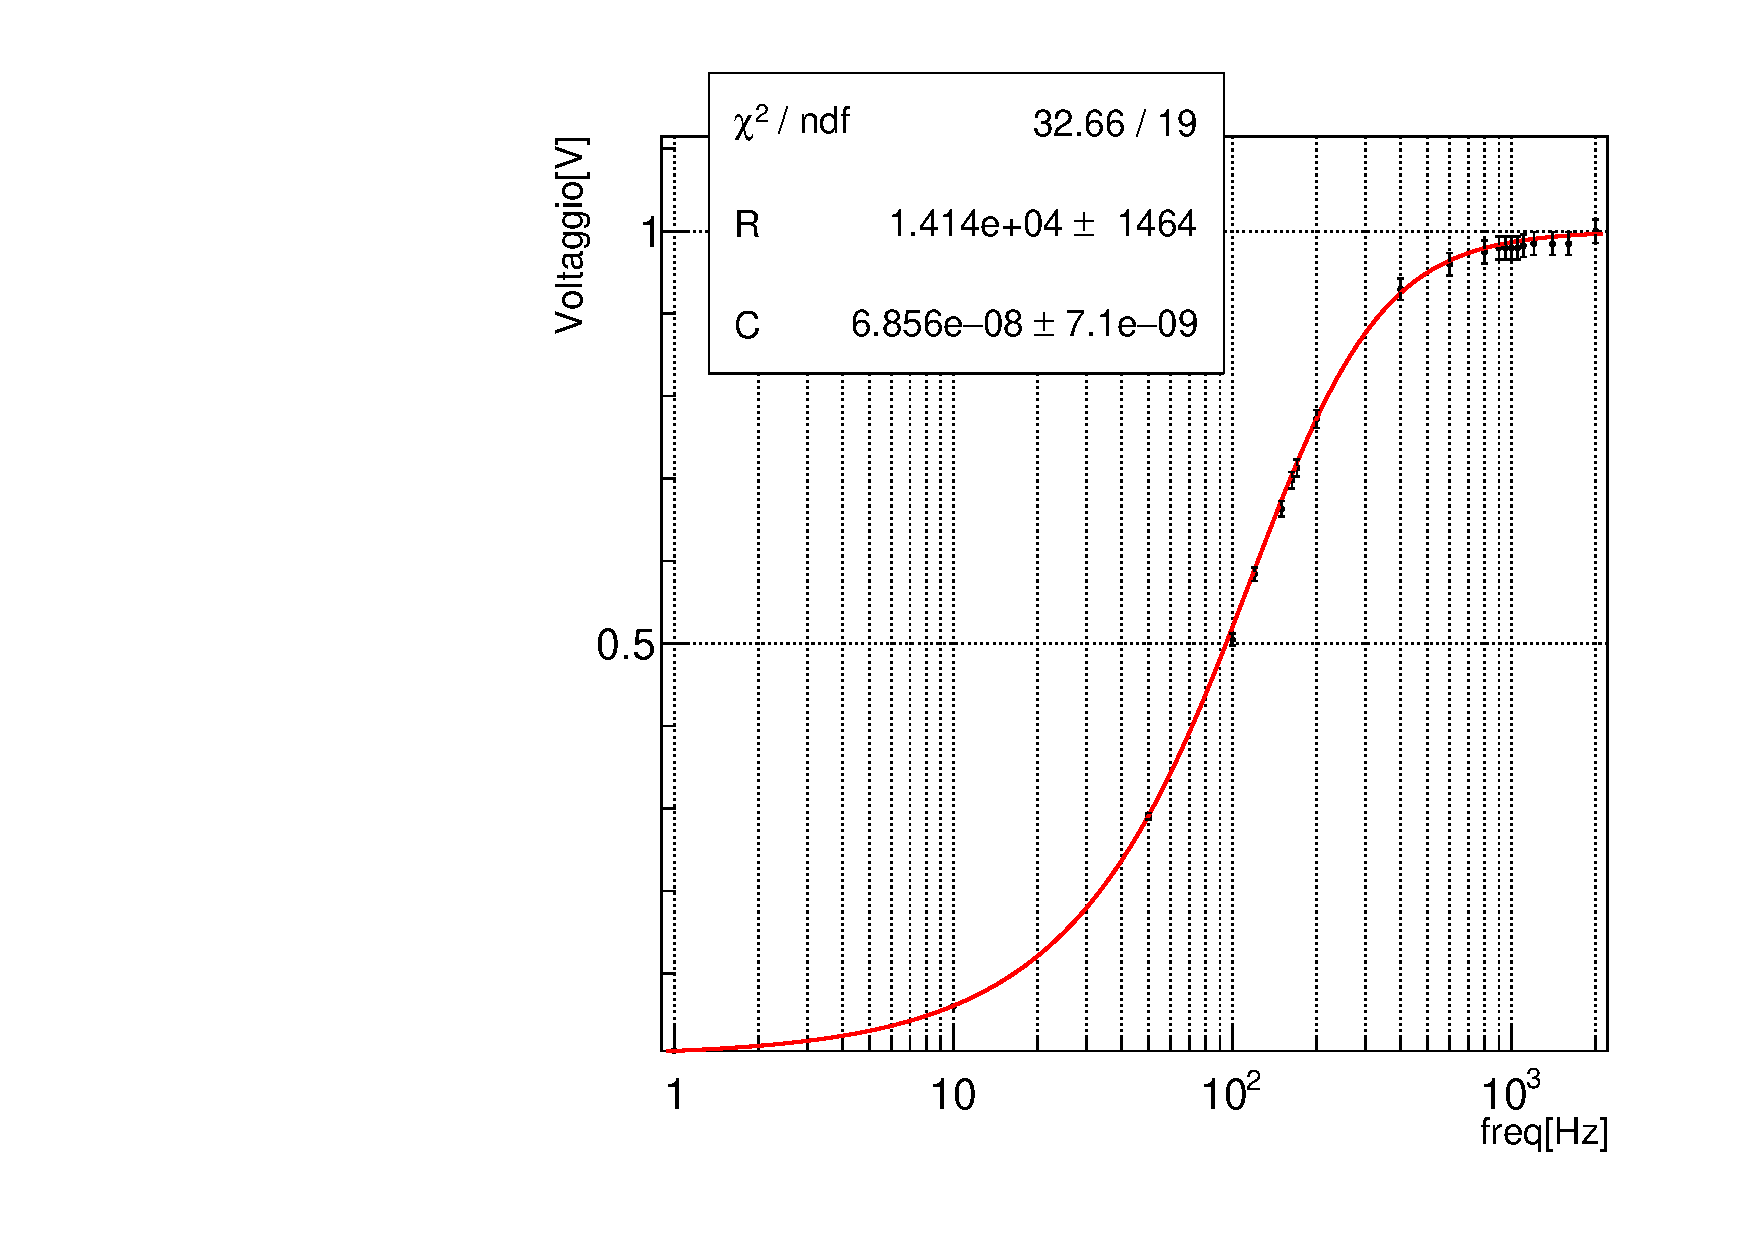
\includegraphics[width=5.7cm]{RC/RC-modulo-capoR.pdf}}
\hfill
\subfigure[fase]{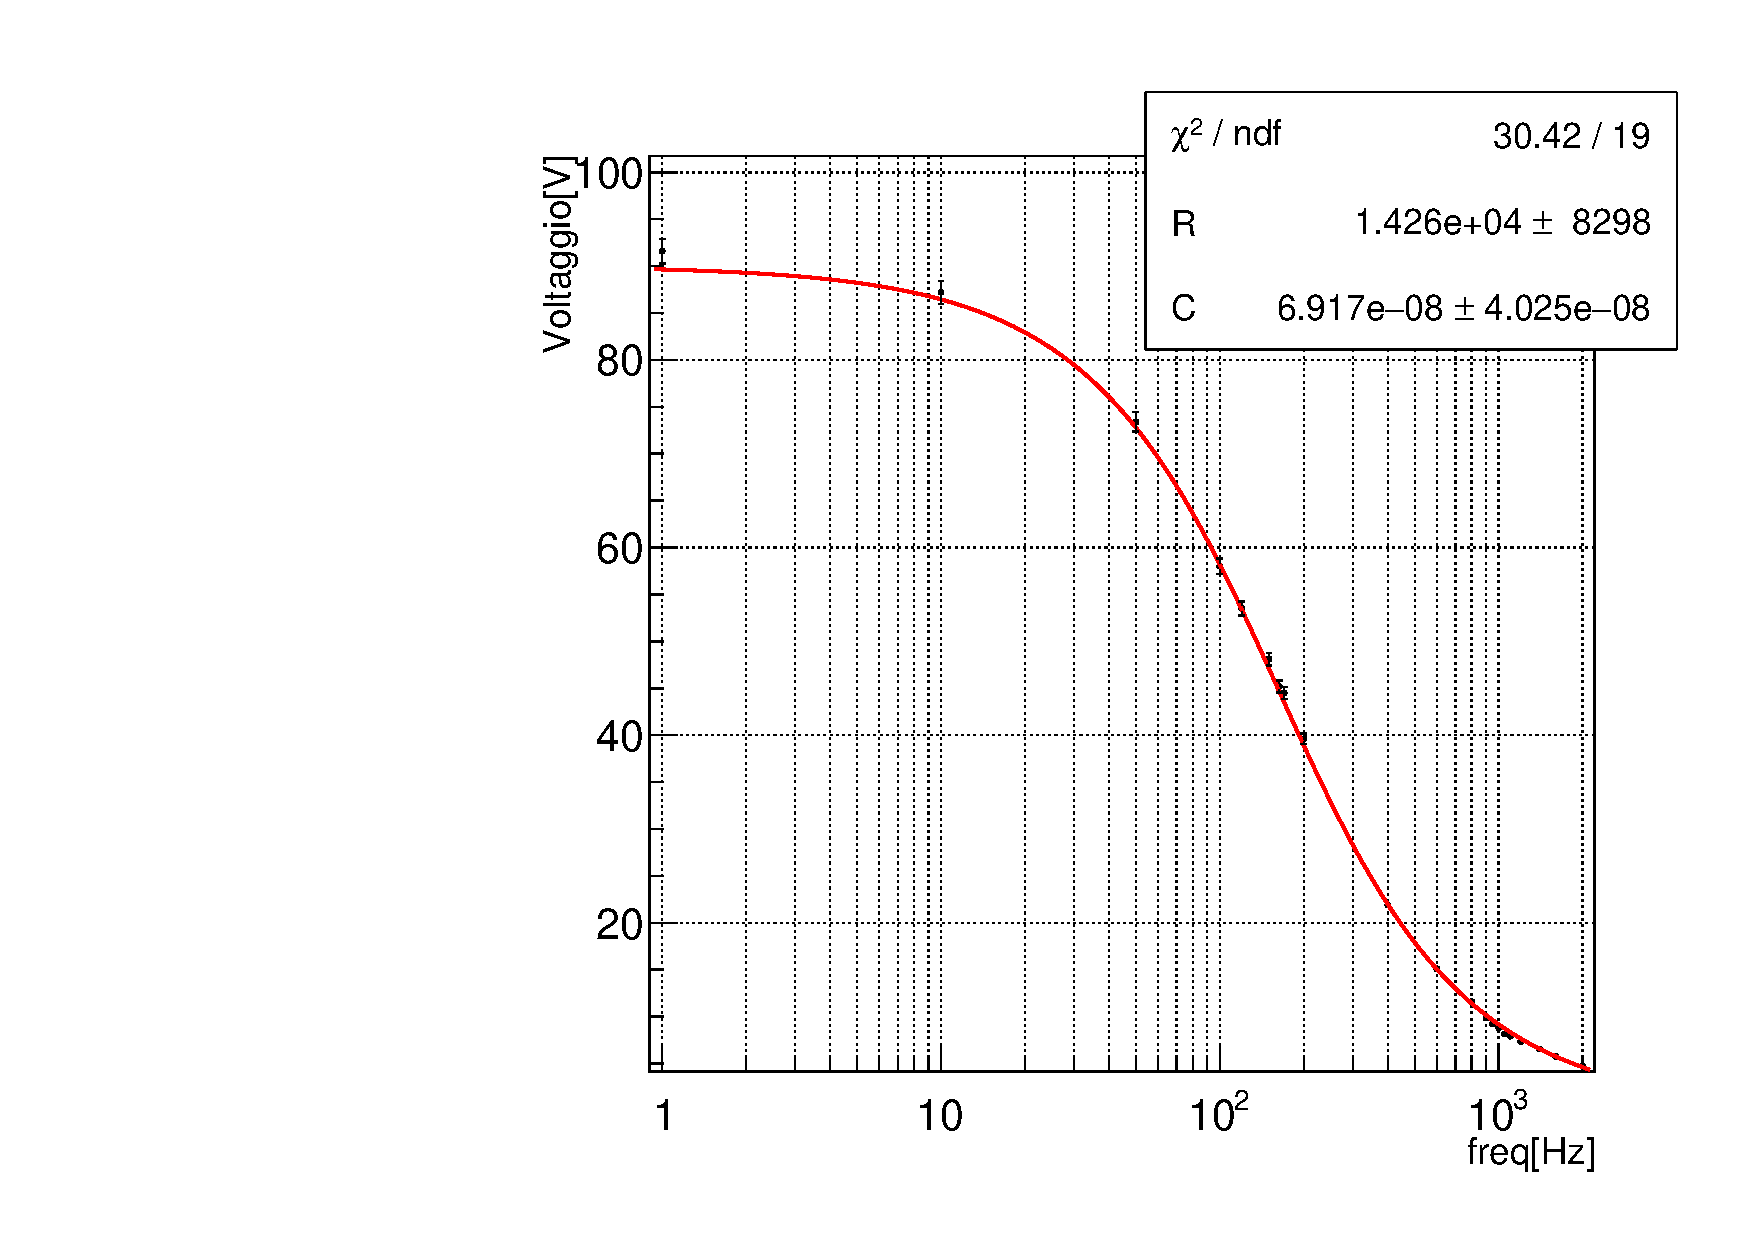
\includegraphics[width=5.7cm]{RC/RC-fase-capoR.pdf}}
\hfill
    }
}
\caption*{osservando la figura (a), notiamo dall'asintoto ad 1 per frequenze alte, che R in un circuito RC agisce da filtro passa alto.}
\label{fig:RC_su_R}
\end{figure}

\noindent Anche in questo caso il test del chi quadro ci permette di notare che abbiamo sottostimato le incertezze associate ai punti, stimiamo che l'errore effettivo sia dato da \(\sqrt{\frac{\chi^{2}}{Ndf}} \cdot \sigma_{V}\) che corrisponde approssimativamente a \(1.3 \cdot \sigma_{V}\) per entrambi i casi.
Le due stime per C ottenute da questa analisi sono le seguenti:

\begin{enumerate}
    \item[-] C dall'interpolazione per il modulo: \(C_{1} = 6.856 \cdot 10^{-8} \pm 0.710 \cdot 10^{-8}\) F
    \item[-] C dall'interpolazione per la fase: \(C_{2} = 6.917 \cdot 10^{-8} \pm 4.025 \cdot 10^{-8}\) F
\end{enumerate}
\noindent che confrontate danno una probabilità di compatibilità del 99.2\%:
\[t = \frac{\left| C_{1} - C_{2}\right|}{\sqrt{\sigma^{2}_{C1} + \sigma^{2}_{C2}}} = 0.01 \rightarrow PValue = 99.2\%\]

\noindent Andiamo a calcolare la media pesata (pesi = \(w_{i} = \frac{1}{\sigma^{2}_{i}}\)) tra le due per ottenere la miglior stima di C: 
\[C_{capoR} = \frac{\sum{C_{i} \cdot w_{i}}}{\sum{w_{i}}}\pm \frac{1}{\sqrt{\sum{w_{i}}}} =  6.858\cdot 10^{-8} \pm 0.699 \cdot 10^{-8} F\]

\noindent Per concludere, le stime per R ottenute sono: 
\begin{enumerate}
    \item[-] R dall'interpolazione per il modulo: \(R_{1} = 14140 \pm 1464 \Omega\)
    \item[-] R dall'interpolazione per la fase: \(R_{2} = 14260 \pm 8298 \Omega \)
\end{enumerate}

\noindent tali stime producono un t = 0.01 che corrisponde alla probabilità di 99.2\%. La media pesata che ne abbiamo ricavato con la formula già riportata sopra è \(R_{capoR} =  14144 \pm 1442  \Omega\).

\subsubsection{Conclusioni sul circuito RC}
Concludiamo l'analisi per questo circuito valutando la compatibilità dei risultati ottenuti ai capi di C ed ai capi di R; abbiamo inoltre effettuato una media pesata delle migliori stime per C ottenute nei paragrafi precedenti in quanto tale valore sarà utile per avviare lo studio del circuito RCL costruito nella seconda parte dell'esperienza.
\begin{enumerate}
    \item[-] \textit{conclusioni su C}\\
    \noindent Date le stime per C: \(C_{capoC} = (6.625 \pm 0.861) \cdot 10^{-8} \) F e \(C_{capoR} = (6.858 \pm 0.699) \cdot 10^{-8} \)F, otteniamo
    \[t = \frac{\left| 6.858 - 6.625\right|}{\sqrt{0.699^{2} + 0.681^{2}}} = 0.2\rightarrow PValue = 84.15\%\]
    \item[-] \textit{conclusioni su R}\\
    \noindent Date le stime per R: \(R_{capoC} = 14007 \pm 1441 \Omega \) e \(R_{capoR} = 14144 \pm 1442 \Omega\), otteniamo
    \[t = \frac{\left| 14144 - 14007 \right|}{\sqrt{1442^{2} + 1441^{2}}} =0.07 \rightarrow PValue = 94.4\%\]
\end{enumerate}

\noindent La miglior stima per C ricavata dall'esperimento con il circuito RC risulta, considerando \(\omega_{capoC} = \frac{1}{\sigma^{2}_{capoC}}\) e \(\omega_{capoR} = \frac{1}{\sigma^{2}_{capoR}}\)

\[C_{RC} = \frac{C_{capoC} \cdot \omega_{capoC} + C_{capoR} \cdot \omega_{capoR}}{\omega_{capoC} + \omega_{capoR}} \pm \frac{1}{\sqrt{\omega_{capoC} + \omega_{capoR}}} = (6.738\pm 0.488) 10^{-8} F\]
\[\Rightarrow C_{RC} \approx 67 \pm 5  nF\]

\pagebreak
\noindent Abbiamo visto come C ed R abbiano, nel nostro caso, compiuto il ruolo rispettivamente di filtro passa basso e filtro passa alto, come annotato sotto le Figure \ref{fig:RC_su_C} e \ref{fig:RC_su_R}; un acuto parallelismo tra il regime CA e le sollecitazioni a tensione quadra ci avrebbe permesso di riconoscere tale proprietà anche dal grafico ottenuto durante l'esperienza Circuiti2. Riportiamo di sotto i grafici della caduta di potenziale ai capi di C e ai capi di R quando il circuito è sollecitato da un'onda quadra:

\begin{figure}[!h]
\caption{ricordiamo da Circuiti2}
\makebox[1 \textwidth][c]{       %centering table
\resizebox{1.20 \textwidth}{!}{   %resize table
\hfill
\subfigure[caduta di potenziale su C]{\includegraphics[width=5.7cm]{RC/crescitaRC (1).pdf}}
\hfill
\subfigure[caduta di potenziale su R]{\includegraphics[width=5.7cm]{RC/decrescitaRC (1).pdf}}
\hfill
    }
}
\caption*{}
\label{fig:RC_daCircuiti2}
\end{figure}

\noindent Durante il fenomeno di carica il circuito era stato sollecitato inizialmente da un potenziale in rapido aumento, che poi è rimasto costante per tutto il processo. La situazione è analoga a un regime CA in cui la frequenza viene inizialmente impostata ad un valore alto e poi abbassata di colpo. Da questa osservazione è facile interpretare i due grafici sopra come:
\begin{enumerate}
    \item[(a)] la caduta di potenziale ai capi di un filtro passa basso (massimo per t \(\gg\) \(\tau\), quindi a basse frequenze) 
    \item[(b)] la caduta di potenziale ai capi di un filtro passa alto (massimo in t = 0, quindi ad alte frequenze)
\end{enumerate}

\pagebreak
\subsection{Circuito RL}
\subsubsection{Funzione di trasferimento su L}
Ancora una volta la funzione di trasferimento si ricava dall'applicazione della legge di Ohm estesa al regime in corrente alternata, che in questo caso scriviamo come:
\[\vec{V}_{L}(t) = \vec{I}(t) \cdot Z_{L} = \frac{\vec{V}_{g}(t) \cdot j\omega L }{r + j\omega L}\]
perciò siccome \(\vec{H} = \frac{\vec{V_{L}}(t)}{\vec{V_{g}}(t)}\), la rappresentazione di \(\vec{H}\) come elemento del campo vettoriale complesso è
\[\vec{H} = \frac{j \omega L}{R + j \omega L}\]

riconosciamo il suo modulo e la sua fase come:
\[ \left| \vec{H} \right| = \frac{\omega L}{\sqrt{R^{2} + (\omega L )^{2}}}\hspace{1cm} (a)\hspace{1cm} \phi_{\vec{H}} = \frac{\pi}{2} - atan\left(\frac{\omega L }{R}\right)\hspace{1cm} (b)\]


\subsubsection*{Dati raccolti}
Per studiare questo circuito abbiamo visualizzato sull'oscilloscopio i potenziali \(\vec{V}_{in}(t)\), \(\vec{V}_{out}(t)\) ai capi di L e \(\vec{V}_{out}(t)\) ai capi di R. \\
I dati sono stati raccolti analogamente a quanto già discusso per il circuito RC, con una medesima stima degli errori strumentali; in base ai risultati del test del chi quadro sulle interpolazioni saremo in grado di valutare l'eventuale presenza di altri errori casuali nel nostro sistema di raccolta. Riportiamo quindi i dati ottenuti per il nuovo circuito:

\begin{table}[!htbp]
\centering
    \captionsetup{labelformat=empty}
    	 \caption{RL - misure ai capi di L}
    \resizebox{12cm}{!}{

    \begin{tabular}{c|c|c|c|c}
        frequenza[Hz] & \(V_{A}\)[V] & \(V_{AB}\)[V] & \(V_{AB}/V_{A}\) & \(\phi_{AB}\)[gradi] \\
        \hline
        \hline
        625      & 20.0 $\pm $ 0.2   & 0.776 $\pm $ 0.008      & 0.0388 $\pm$ 0.0004\\
        1250     & 20.0 $\pm $ 0.2   & 1.10 $\pm $ 0.01          & 0.0550 $\pm$ 0.0006 & 86 $\pm$ 1 \\
        2500     & 20.0 $ \pm$ 0.2   & 2.35 $\pm $ 0.02        & 0.118 $\pm$ 0.001& 86 $\pm$ 1\\
        5000     & 20.0 $ \pm$ 0.2   & 4.70 $\pm $ 0.05   & 0.235 $\pm$ 0.003 & 75 $\pm$ 1 \\
        10000    & 20.0 $ \pm$ 0.2   & 8.50 $\pm $ 0.09    & 0.425 $\pm$ 0.005 & 71 $\pm$ 1    \\
        20000    & 20.0 $\pm $ 0.2   & 13.5 $\pm $ 0.1        & 0.675 $\pm$ 0.008& 50.5 $\pm$ 0.7  \\
        40000    & 20.0 $\pm $ 0.2   & 17.5 $\pm $ 0.2     & 0.88 $\pm$ 0.01 & 28.5 $\pm$ 0.4\\
        80000    & 20.0 $\pm $ 0.2   & 19.4 $ \pm$ 0.2         & 0.97 $\pm$ 0.01& 15.2 $\pm$ 0.2 \\
        160000   & 20.2 $\pm $ 0.2 & 20 $ \pm$ 0.2     & 0.99 $\pm$ 0.01 & 6.9 $\pm$ 0.1\\
        \hline
        \hline
    \end{tabular}
    }
\caption{errore strumentale: 1\%}
\caption{Nota: le misure per \(\phi_{AB}\) e \(\phi_{B}\) relative a 625Hz non sono state riportate poichè lo strumento restituiva numerosi valori inconsistenti, quindi da noi ritenuti non significativi. }
\end{table}


\subsubsection*{Analisi dati}
Lo studio effettuato sui dati sopra riportati parte ancora una volta dall'esecuzione del fit con il modello atteso per il modulo di H e la sua fase. Di sotto riportiamo i grafici ottenuti dalle interpolazioni del caso. \\

\begin{figure}[!h]
\caption{RL - funzione di trasferimento ai capi di L}
\makebox[1 \textwidth][c]{       %centering table
\resizebox{1.30 \textwidth}{!}{   %resize table
\hfill
\subfigure[modulo]{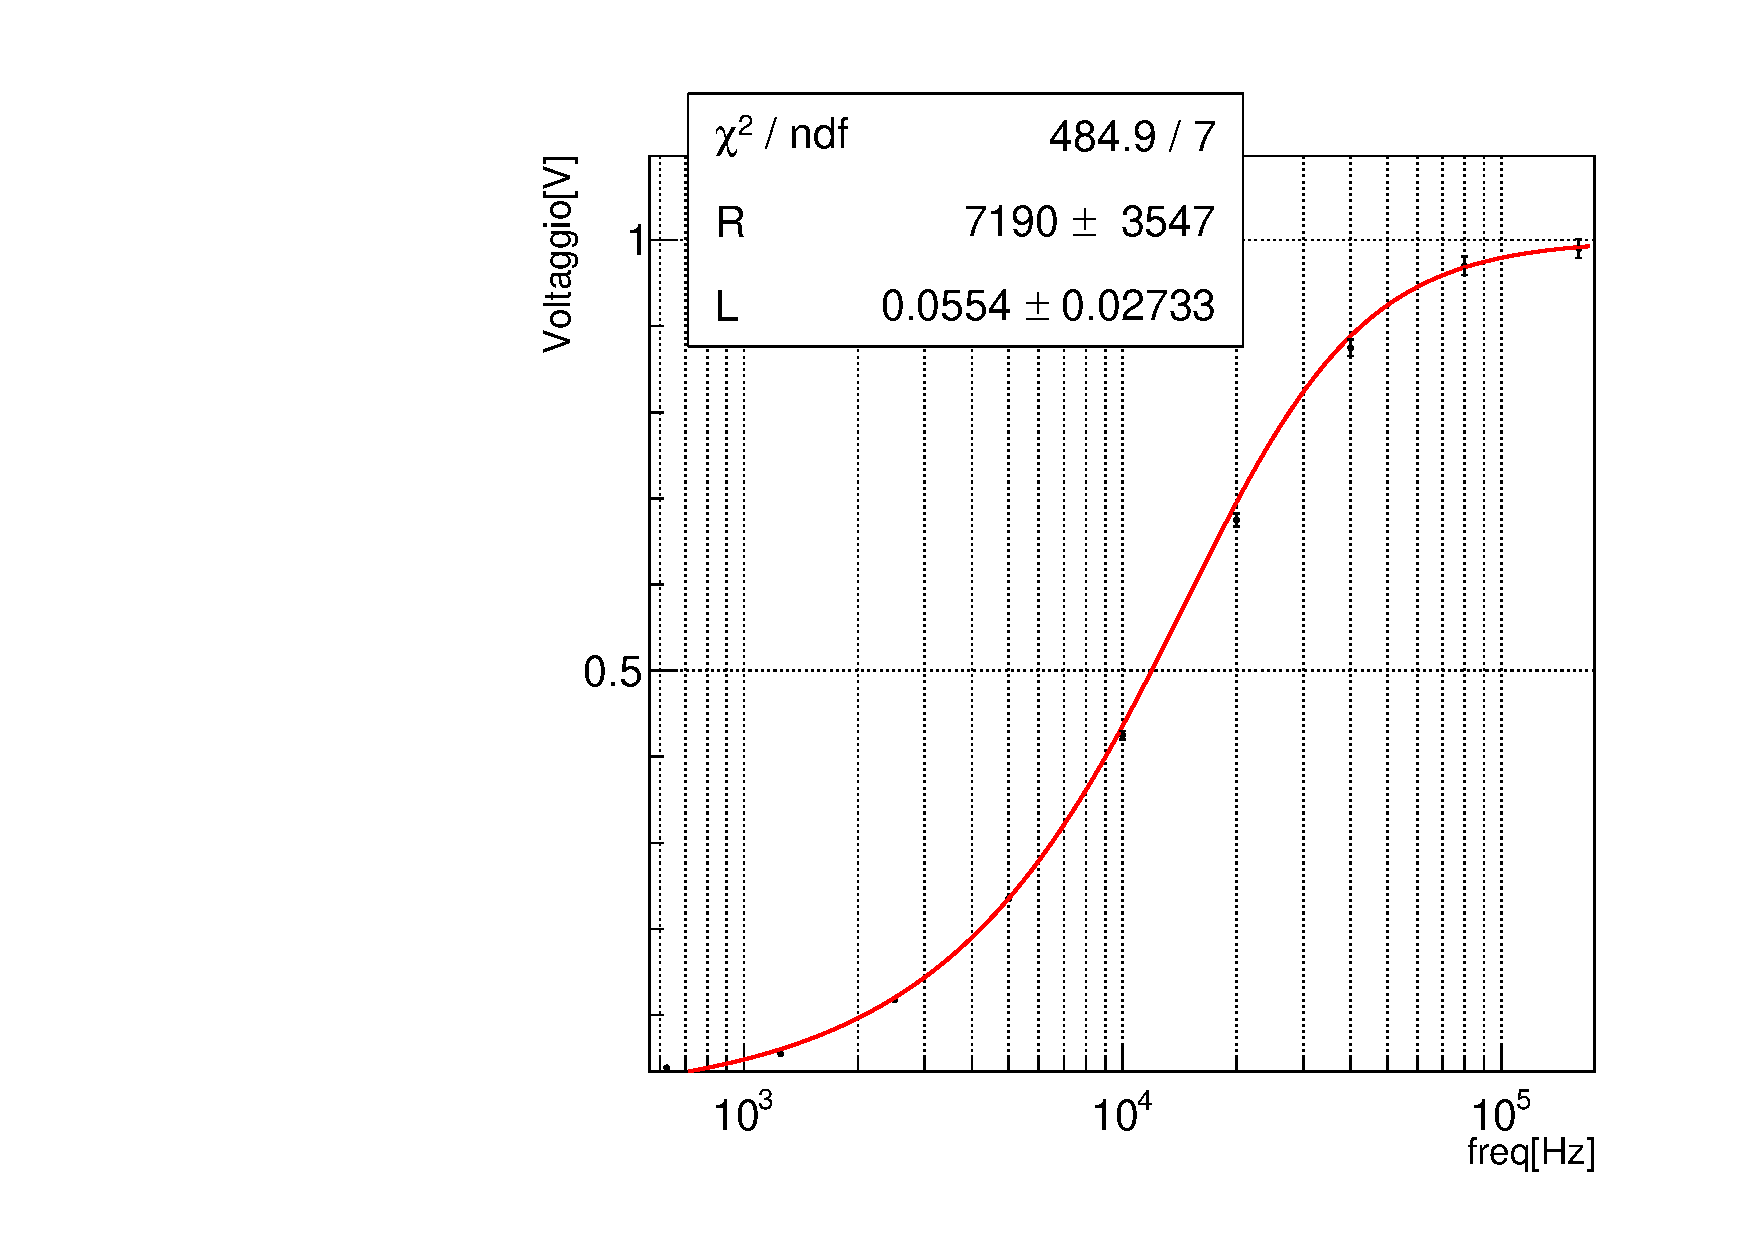
\includegraphics[width=5.7cm]{RL/RL-modulo-capoL.pdf}}
\hfill
\subfigure[fase]{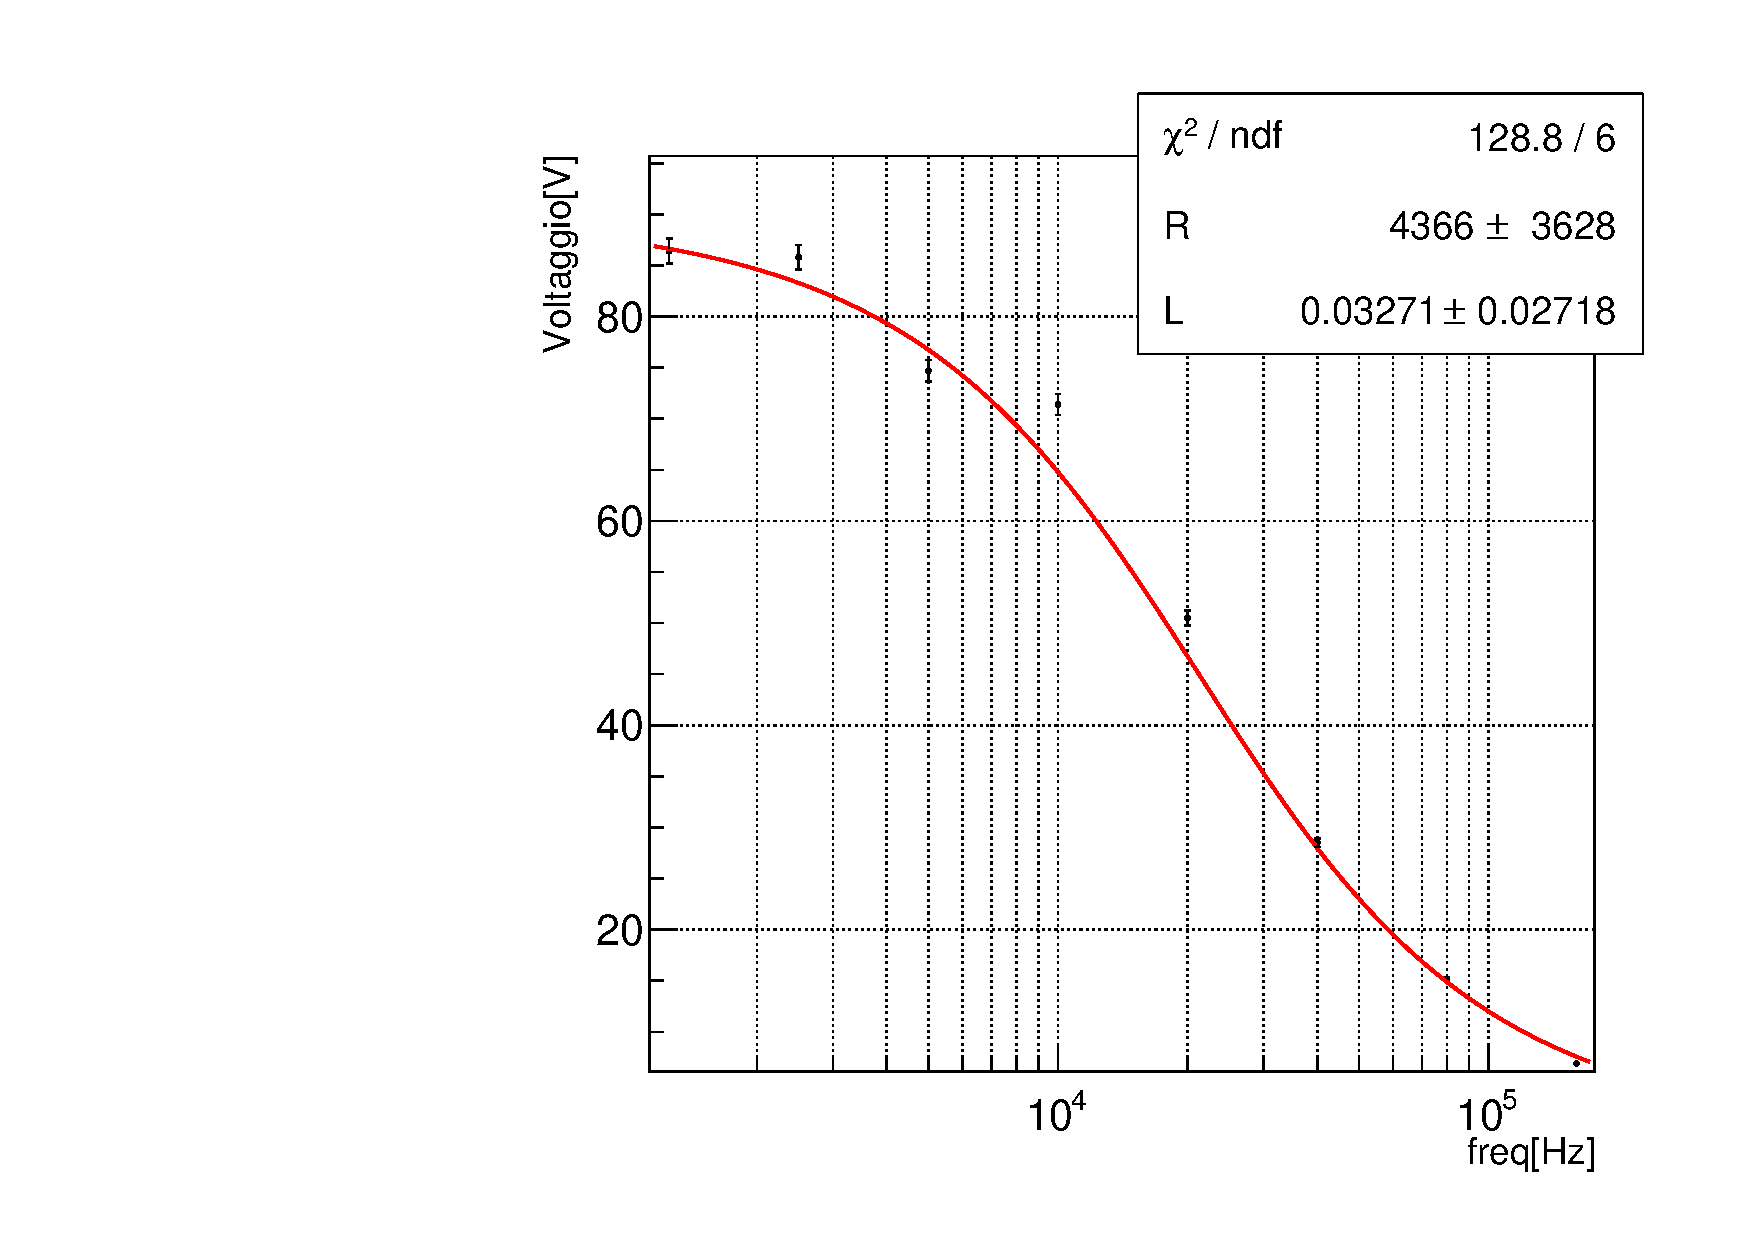
\includegraphics[width=5.7cm]{RL/RL-fase-capoL.pdf}}
\hfill
    }
}
\label{fig:RL_su_L}
\caption*{osservando la figura (a), dall'asintoto a 1 per frequenze alte si può notare come l'induttanza di un circuito RL compia il ruolo di filtro passa alto.}
\end{figure}

\noindent I dati rispettano gli andamenti attesi, tuttavia in entrambi i casi il test del chi quadro non restituisce risultato accettabile, il che porta a supporre di aver trascurato la presenza di ulteriori errori casuali che possono aver portato a maggiori fluttuazioni delle misure rispetto a quelle previste. Una possibilità che prendiamo in considerazione è che tale rumore sia di origine termica, quindi da associare alla resistenza interna dell'induttanza che essendo pittosto piccola, almeno per frequenze basse, è soggetta all'attraversamento di grandi quantità di corrente. \\\\
Associamo quindi il fallimento del test sull'interpolazione del modulo ad una sottostima degli errori sulle prime misure, quelle affette maggiormente dal rumore termico. \\
Per quanto riguarda la fase notiamo ancora che le misure relative a frequenze basse sono molto meno accurate delle ultime, come potevamo aspettarci dal momento che il rumore sui tempi  \(\sigma_{t}\) in un grafico V(t) è proporzionale al rumore sul voltaggio \(\sigma_{V}\) secondo:
\[\sigma_{t} \propto \frac{\sigma_{V}}{\frac{dV}{dt}}\]
perciò ad errori maggiori su V corrispondono errori maggiori anche sui tempi, da cui la stima di \(\phi\) dipende necessariamente. \\\\
Questo esperimento ci ha permesso di ricavare due stime per L che possiamo mettere a confronto con il test t-Student: \\
\begin{enumerate}
    \item[-] L dall'interpolazione per il modulo: \(L_{1} = 0.0554 \pm 0.0273H\)
    \item[-] L dall'interpolazione per la fase: \(L_{2} = 0.0327 \pm 0.0272 H\)
\end{enumerate}
\[t = \frac{\left|L_{1} - L_{2}\right|}{\sqrt{\sigma^{2}_{L1} + \sigma^{2}_{L2}}} = 0.6 \rightarrow PValue = 54.85\%\]

\noindent Dopo aver trovato due valori statisticamente compatibili fra loro abbiamo calcolato la loro media pesata come:
\[L_{capoL} = \frac{\sum{L_{i} \cdot w_{i}}}{\sum{w_{i}}}\pm \frac{1}{\sqrt{\sum{w_{i}}}} = 0.0440 \pm 0.0193 H\]

\noindent Analizziamo anche le stime ottenute per R dalle due interpolazioni:
\begin{enumerate}
    \item[-] R dall'interpolazione sul modulo: \(R_{1} =  7190\pm 3547\Omega \)
    \item[-] R dall'interpolazione sulla fase: \(R_{2} =  4366\pm  3628\Omega\)
\end{enumerate}

\noindent dal loro confronto tramite il test t-Student otteniamo:
\[t = \frac{\left| R_{1} - R_{2}\right|}{\sqrt{\sigma^{2}_{R1} + \sigma^{2}_{R2}}} = 0.6 \rightarrow PValue = 54.85\%\]
\noindent Abbiamo eseguito una media pesata con la formula già riportata sopra, ottendendo il valore di \( R_{capoL} =  4378 \pm 2536 \Omega\).

\pagebreak
\subsubsection{Funzione di trasferimento su R}
Ricaviamo la funzione di trasferimento ai capi di R come segue:
\[\vec{V}_{R}(t) = \vec{I}(t) \cdot R = \frac{V_{g}(t) \cdot R}{R + j\omega L}\]
\[\Downarrow\]
\[\vec{H} = \frac{R}{R + j \omega L}\]
da cui riconosciamo il suo modulo e la sua fase: 
\[\left|\vec{H} \right| = \frac{R}{\sqrt{R^{2} + (\omega L)^{2}}}\hspace{1cm} (a)\hspace{1cm} \phi_{\vec{H}} = 0 - atan\left(\frac{\omega L }{R}\right)\hspace{1cm} (b) \]

\subsubsection*{Dati raccolti}
Le misure ottenute per ampiezza e fase ai capi di R sono le seguenti:

\begin{table}[!htbp]
\centering
    \captionsetup{labelformat=empty}
    	 \caption{RL - misure ai capi di R}
    \resizebox{12cm}{!}{

    \begin{tabular}{c|c|c|c|c}
        frequenza[Hz] & \(V_{A}\)[V] & \(V_{B}\)[V] & \(V_{B}/V_{A}\) & \(\phi_{B}\)[gradi] \\
        \hline
        \hline
        
        625     & 20.0 $\pm $ 0.2    & 20.0 $\pm $ 0.2    & 1.00 $ \pm$ 0.01\\
        1250    & 20.0 $\pm $ 0.2    & 20.0 $\pm $ 0.2    & 1.00 $\pm $ 0.01& -3.60 $\pm$ 0.05\\
        2500    & 20.0 $\pm $ 0.2    & 19.6 $ \pm$ 0.2        & 0.98 $ \pm$ 0.01& -4.50 $\pm$ 0.06\\
        5000    & 20.0 $\pm $ 0.2    & 19.6 $ \pm$ 0.2        & 0.98 $\pm $ 0.01 & -8.6 $\pm$ 0.1\\
        10000   & 20.0 $\pm $ 0.2    & 18.8 $\pm $ 0.2        & 0.94 $\pm $ 0.01& -17.3 $\pm$ 0.2\\
        20000   & 20.0 $\pm $ 0.2    & 16.8 $\pm $ 0.2        & 0.84 $\pm $ 0.01   & -31.7 $\pm$ 0.4\\
        40000   & 20.0 $\pm $ 0.2    & 12.4 $\pm $ 0.1        & 0.620 $\pm $ 0.009   & -51.8 $\pm$ 0.7\\
        80000   & 20.0 $\pm $ 0.2    & 6.88 $\pm $ 0.07       & 0.344 $\pm $ 0.005   & -69 $\pm$ 1\\
        160000  & 20.2 $\pm $ 0.2& 3.56 $ \pm$ 0.04 & 0.176$\pm $ 0.002& -81 $\pm$ 1\\
        \hline
        \hline
    \end{tabular}
    }
\caption{errore strumentale: 1\%}
\end{table}

\pagebreak
\subsubsection*{Analisi dati}
Abbiamo eseguito l'interpolazione dei grafici ottenuti similmente a come già spiegato e osservato il seguente risultato: 

\begin{figure}[!h]
\caption{RL - funzione di trasferimento ai capi di R}
    \makebox[1 \textwidth][c]{       %centering table
	\resizebox{1.10 \textwidth}{!}{   %resize table
\hfill
\subfigure[modulo]{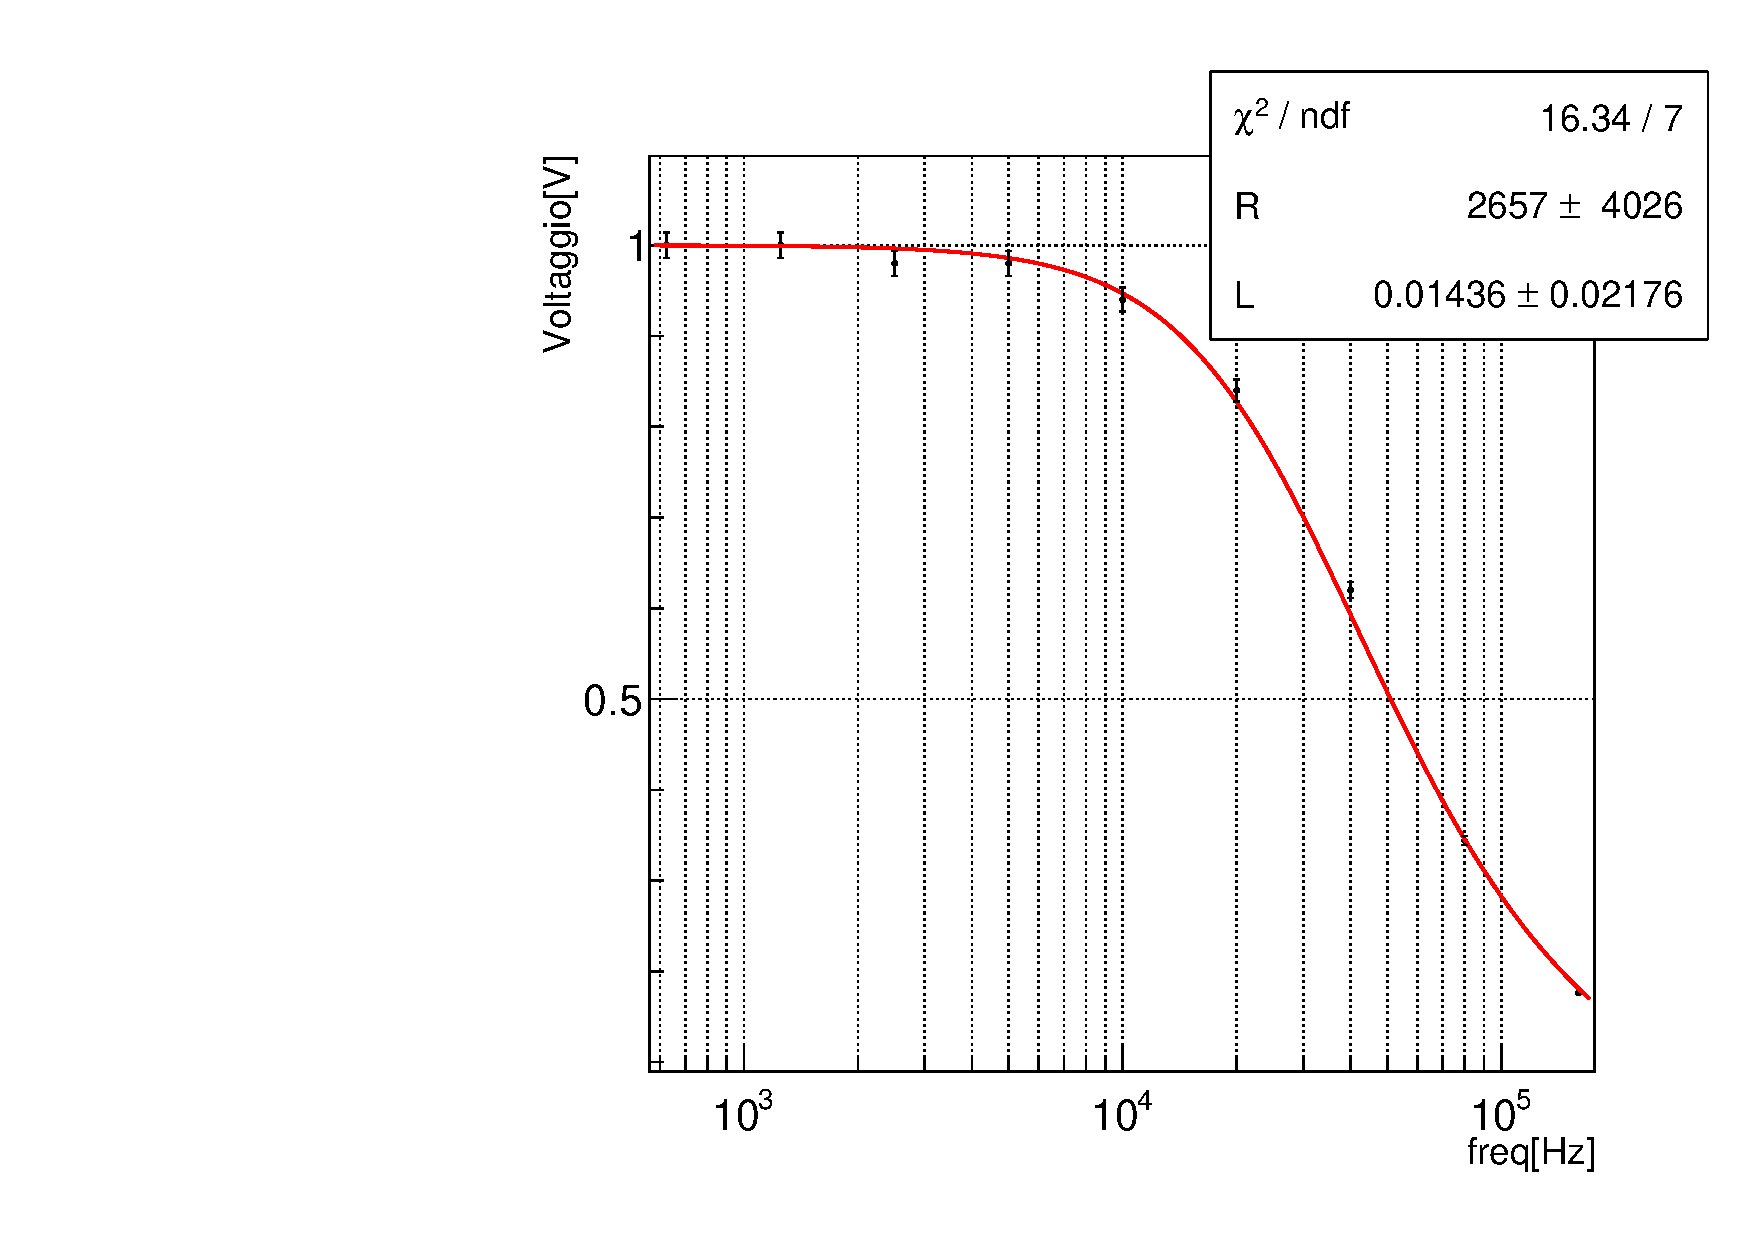
\includegraphics[width=5.8cm]{RL/RL-modulo-capoR.pdf}}
\hfill
\subfigure[fase]{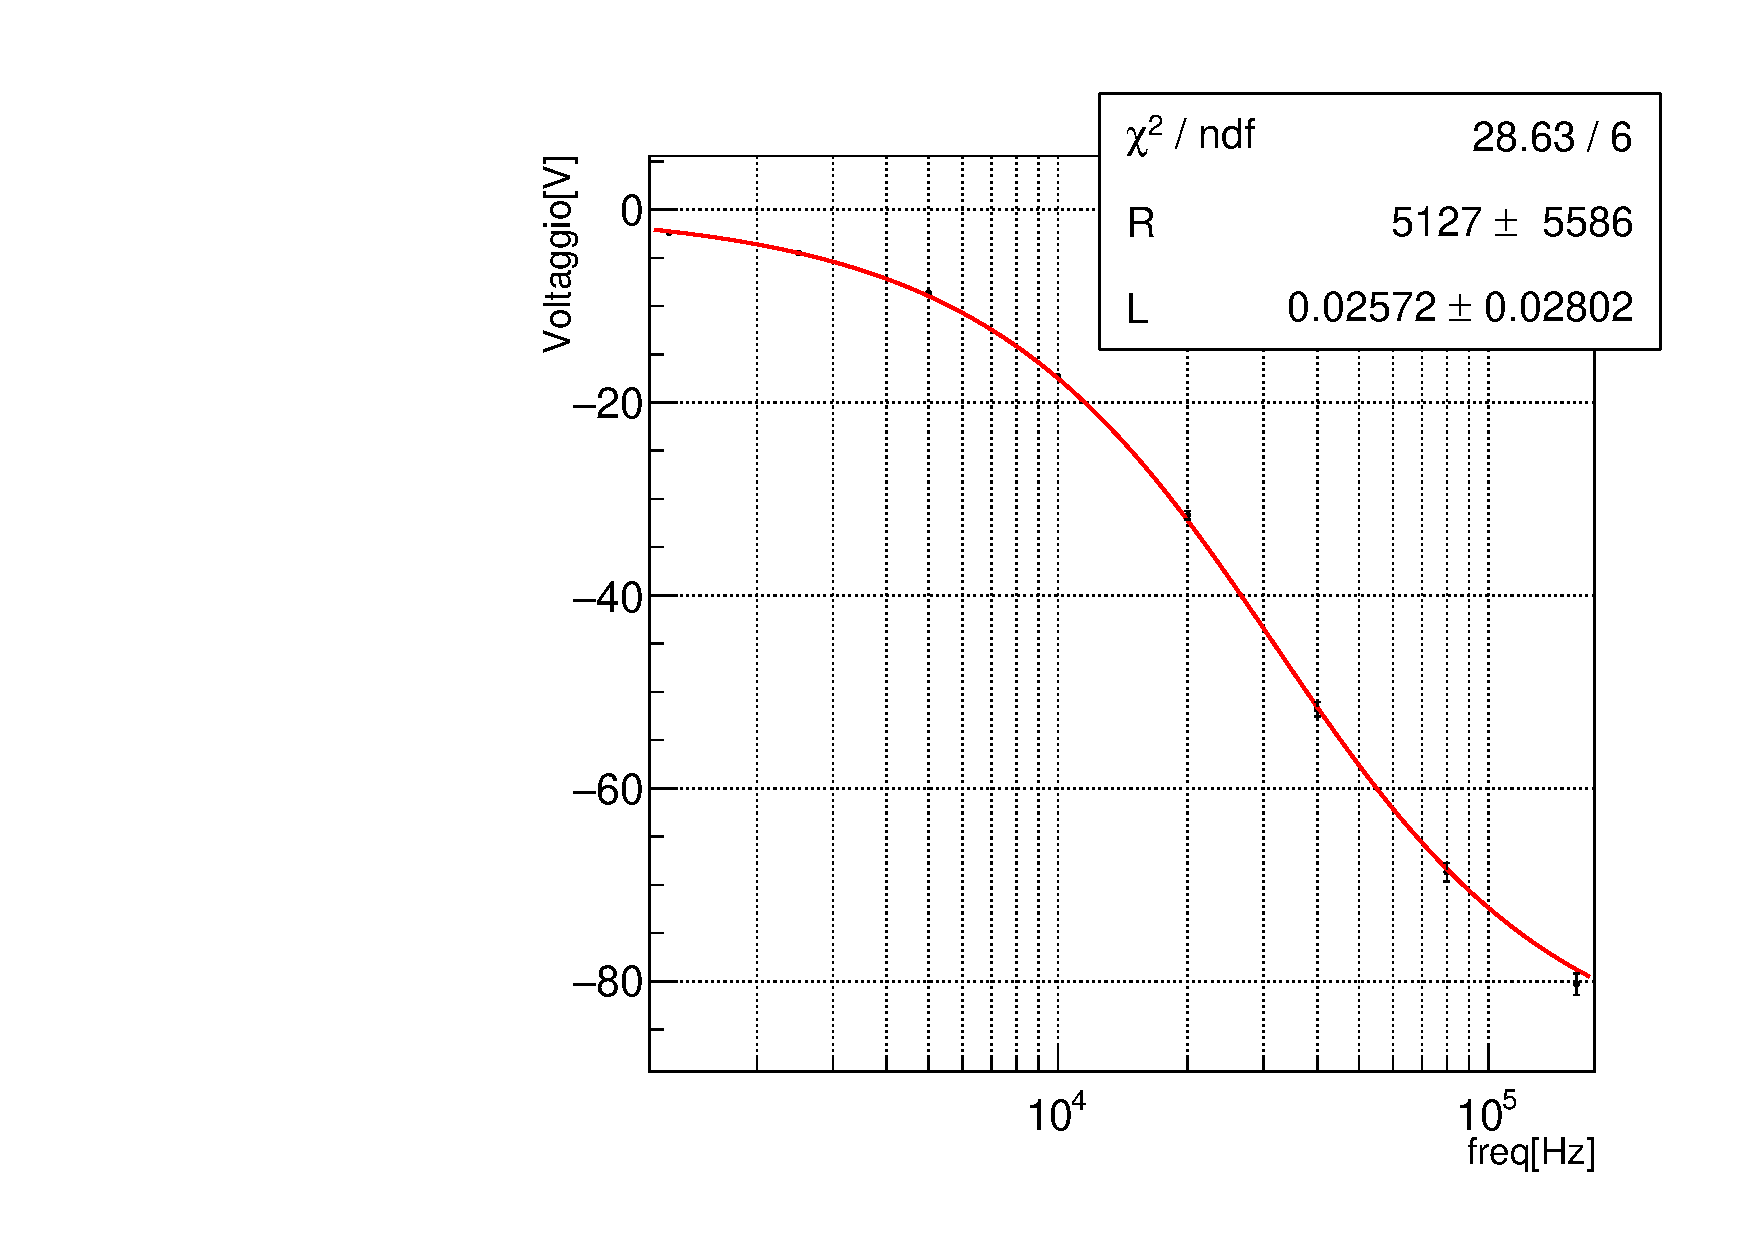
\includegraphics[width=5.8cm]{RL/RL-fase-capoR.pdf}}
\hfill
    }
}
\label{fig:RL_su_R}
\caption*{si osservi la figura (a), dal passaggio per 1 a frequenze basse si deduce come la resistenza del circuito RL operi da filtro passa basso.}

\end{figure}

\noindent Osserviamo che questa volta per il modulo di H il test del chi quadro riporta una probabilità accettabile del 5\% che il modello soggiacente al fenomeno osservato sia quello atteso, tuttavia essendo il rapporto \(\frac{16.34}{7} = 2 > 1\) supponiamo di aver trascurato una fonte di errori casuali che ha portato ad aumentare l'incertezza effettiva sulle misure. Questa fonte è possibile sia il resistore stesso ai capi del quale stiamo misurando il potenziale in uscita che, scaldandosi, accentua il moto browniano dei portatori di carica al suo interno creando quello che chiamiamo rumore termico. Una situazione simile si riconosce anche nell'analisi delle misure per la fase, dove abbiamo \(\chi^{2} =28.63 \) e Ndf = 6, il test non restituisce un valore accettabile per la probabilità ma associamo a questo insuccesso la sottostima delle incertezze già precedentemente discussa. \\

\noindent Le due stime per L ottenute da questa analisi sono le seguenti:
\begin{enumerate}
    \item[-] L dall'interpolazione per il modulo: \(L_{1} = 0.0144 \pm 0.0218 H\)
    \item[-] L dall'interpolazione per la fase: \(L_{2} = 0.0257 \pm 0.0280 H\)
\end{enumerate}
\noindent che confrontate danno una probabilità di compatibilità del 76.4\%:
\[t = \frac{\left| L_{1} - L_{2}\right|}{\sqrt{\sigma^{2}_{L1} + \sigma^{2}_{L2}}} = 0.3 \rightarrow PValue = 76.4\%\]

\noindent Andiamo a calcolare la media pesata (pesi = \(w_{i} = \frac{1}{\sigma^{2}_{i}}\)) tra le due per ottemere la miglior stima di ai capi di R: 
\[L_{capoR} = \frac{\sum{L_{i} \cdot w_{i}}}{\sum{w_{i}}}\pm \frac{1}{\sqrt{\sum{w_{i}}}} = 0.0187 \pm 0.0172 H\]

\noindent Controlliamo anche le stime per R che sono:
\begin{enumerate}
    \item[-] R dall'interpolazione sul modulo: \(R_{1} = 2657 \pm 4026 \Omega \)
    \item[-] R dall'interpolazione sulla fase: \(R_{2} = 5127 \pm 5586 \Omega\)
\end{enumerate}

\noindent dal loro confronto tramite il test t-Student otteniamo:
\[t = \frac{\left| R_{1} - R_{2}\right|}{\sqrt{\sigma^{2}_{R1} + \sigma^{2}_{R2}}} = 0.4 \rightarrow PValue = 68.9\%\]
\noindent Abbiamo inoltre eseguito una media pesata tra i due valori per R ottenuti ai capi di R per ottenere, con la formula già riportata sopra, un valore di \(R_{capoR} =  3501 \pm 580 \Omega\).


\subsubsection{Conclusioni sul circuito RL}
\noindent Abbiamo notato che per il circuito RL i valori degli errori sulle stime ottenute di R ed L sono paragonabili o addirittura maggiori dei valori stessi delle stime. Questa mancanza di precisione è probabilmente dovuta alle poche misure effettuate in quanto, pur avendo raccolto il doppio dei dati in laboratorio, ci siamo accorti che le frequenze impostate per ricavare le misure finali erano fin troppo alte poichè hanno causato un comportamento anomalo del circuito. Infatti per frequenze alte l'induttanza tende a comportarsi come una resistenza e per la sua capacità di immagazzinare energia diventa sempre più trascurabile. Tenendo conto anticipatamente di questa considerazione avremmo potuto infittire il campionamento nel range di frequenze effettivamente significative. \\

\noindent Per concludere l'analisi dati relativa a questo circuito valutiamo la compatibilità delle due medie pesate per L ottenute nei paragrafi precedenti e in caso effettuiamo una media complessiva, sarà utile nel valutare le proprietà del circuito RCL che abbiamo costruito per la seconda parte. \\
\begin{enumerate}
    \item[-]\textit{conclusioni su L}\\
    \noindent Date le stime per L: \(L_{capoL} = 0.0440 \pm 0.0193\)H e \(L_{capoR} = 0.0187 \pm  0.0172\)H, otteniamo:
\[t = \frac{\left| 0.0440 - 0.0187 \right|}{\sqrt{0.0193^{2} + 0.0172^{2}}} = 1 \rightarrow PValue = 31.73\%\]

    \item[-]\textit{conclusioni su R}\\
    \noindent Date le stime per R: \(R_{capoL} = 4378 \pm 2536 \Omega\) e \(R_{capoR} = 3501 \pm 580 \Omega\), otteniamo:
\[t = \frac{\left| 4378 - 3501  \right|}{\sqrt{2563^{2} + 580^{2}}} = 0.3 \rightarrow PValue = 76.42 \%\]
\end{enumerate}


\noindent La miglior stima per L ricavata dall'esperimento con il circuito RL  risulta, considerando \(w_{capoL} = \frac{1}{\sigma^{2}_{capoL}}\) e \(w_{capoR} = \frac{1}{\sigma^{2}_{capoR}}\)

\[L_{RL} = \frac{L_{capoL}\cdot w_{capoL}+ L_{capoR}\cdot w_{capoR}}{w_{capoL} + w_{capoR}} \pm \frac{1}{\sqrt{w_{capoL} + w_{capoR}}} = 0.0327 \pm 0.0134 H \]
\[\Rightarrow  L_{RL}\approx 0.03 \pm 0.01 H\]

\noindent Si osservi che è assolutamente lecito eseguire un parallelismo analogo a quello effettuato tra il circuito RC in corrente impulsata e quello in corrente alternata anche per il circuito RL, analisi che qui non riportiamo perchè potrebbe essere ripetitiva. 

\section{Parte seconda}
Nella seconda giornata in laboratorio abbiamo studiato il trasferimento del segnale alternato attraverso circuiti che comprendono tutti i componenti studiati fin'ora: R, C ed L. Nonostante abbiamo cercato di selezionare componenti dai valori simili a quelli utilizzati per lo svolgimento della prima parte, non riteniamo ragionevole effettuare confronti con i parametri ottenuti in questa parte. \\
I valori attesi per le relative impedenze sono i medesimi già riportati nella Parte prima. 

\subsection{Procedimento adottato}
Lo schema del circuito costruito ed una foto della sua realizzazione in laboratorio sono riportati in figura \ref{fig:RCL-schema-e-foto}. Ai fini della rappresentazione di modulo e fase della funzione H ai capi di ciascun componente è stato necessario invertire ogni volta i componenti di modo che quello interessato si trovasse tra la sonda che misura l'uscita e la massa, quello rappresentato in figura è un esempio di circuito LCR, adoperato per studiare H ai capi di R. \\
\noindent Per questa parte è duque stato sufficiente visualizzare \(\vec{V}_{in}\) e \(\vec{V}_{out}\) ai capi del componente interessato per misurare le ampiezze picco-picco \(V_{A}\) e \(V_{B}\) e la fase \(\phi_{B}\) di \(\vec{V}_{out}\) rispetto a \(\vec{V}_{in}\).  \\\\\\\\

\begin{figure}[!h]
\caption{esempio di un circuito LCR}

\makebox[1 \textwidth][c]{       %centering table
\resizebox{1.0 \textwidth}{!}{   %resize table
\hfill
\subfigure[schema]{\includegraphics[width=5.7cm]{RLC/LCR-schema.png}}
\hfill
\subfigure[realizzazione in laboratorio]{\includegraphics[width=5.7cm]{RLC/LCRfoto.jpeg}}
\hfill
    }
}
\label{fig:RCL-schema-e-foto}
\end{figure}

\noindent Per avere una stima in termini di ordini di grandezza delle frequenze attorno cui campionare il grafico abbiamo sfruttato il concetto di frequenza di risonanza\footnote{frequenza alla quale le componenti reattive di Z si equivalgono in modulo e, pertanto, avendo segno opposto si annullano reciprocamente} ed adoperato le stime ottenute nella prima parte. Sappiamo infatti che il grafico del modulo della funzione H potrebbe presentare un picco in corrispondenza di \(f = \frac{1}{2\pi\sqrt{LC}} \approx 3550 Hz\).

\subsection{Circuiti LCR - RLC - RCL}
\subsubsection{Funzione di trasferimento su R}
Anche per questa situazione, ci siamo ricavati la funzione di trasferimento partendo dalla legge di Ohm.
\[\vec{V}_{R}(t)= \vec{I}(t) \cdot R = \frac{R \cdot \vec{V}_{g}}{R+jwL-\frac{1}{jwC}}\]

\[\Downarrow\]

\[\vec{H} = \frac{R}{R+jwL-\frac{1}{jwC}} \]
scriviamo quindi modulo e fase come:
\[\left|\vec{H}\right|=\frac{RwC}{\sqrt{w^{2} C^{2} R^{2} +(w^{2}LC-1)^{2}}}\hspace{1cm} (a) \hspace{1cm} \phi_{\vec{H}}= 0 - \arctan\left(\frac{wL-\frac{1}{wC}}{R}\right)\hspace{1cm} (b)\]
funzioni che abbiamo utilizzato per eseguire le interpolazioni del caso sempre sostituendo \(2 \pi x\) a \(\omega\). 

\pagebreak
\subsubsection*{Dati raccolti}
Visualizzando sull'oscilloscopio \(\vec{V}_{in}\) e \(\vec{V}_{out}\) ai capi di R abbiamo raccolto il primo set di dati al variare della frequenza. Per i valori associati a \(V_{B}\), ovvero l'ampiezza picco-picco di \(\vec{V}_{out}\), \(V_{A}\), ovvero l'ampiezza picco-picco di \(\vec{V}_{in}\) e \(\phi_{B}\), l'analisi degli errori strumentali eseguita nel paragrafo per il circuito RC rimane valida. 

\begin{table}[!htbp]
\centering
    \captionsetup{labelformat=empty}
    	 \caption{CLR - misure ai capi di R}
    \resizebox{13.5cm}{!}{

    \begin{tabular}{c|c|c|c|c}
        frequenza[Hz] & \(V_{A}\)[V] & \(V_{B}\)[V] & \(V_{B}/V_{A}\) & \(\phi_{B}\)[gradi] \\
        \hline
        \hline
        10      & 20.4 $ \pm$ 0.2      & 0.124 $ \pm $ 0.001 & 0.00608 $ \pm $ 0.00009 & 90 $\pm$ 1\\
        50      & 20.4 $ \pm $ 0.2  & 0.612 $ \pm $ 0.006& 0.0300 $ \pm $ 0.0004& 88 $\pm$ 1\\
        100     & 20.4 $  \pm$ 0.2    & 1.23 $ \pm $ 0.01 & 0.0603 $ \pm $ 0.0009 & 85 $\pm$ 1\\
        250     & 20.4 $ \pm $ 0.2& 3.50 $ \pm $ 0.04 & 0.172 $ \pm $ 0.002 & 81 $\pm$ 1\\
        500     & 20.4 $  \pm$ 0.2& 6.32 $ \pm $ 0.06  & 0.310 $  \pm$ 0.004& 70 $\pm$ 1\\
        1000    & 19.8 $ \pm $ 0.2     & 13.0 $  \pm$ 0.1 & 0.657 $ \pm $ 0.009& 44.3 $\pm$ 0.6\\
        2000    & 19.4 $ \pm $ 0.2       & 17.0 $ \pm $ 0.2  & 0.88 $ \pm $ 0.01& -15.9 $\pm$ 0.2\\
        5000    & 20.0 $ \pm $ 0.2    & 7.26 $ \pm $ 0.07     & 0.363 $ \pm $ 0.005& -67.0 $\pm$ 0.9 \\
        10000   & 20.4 $ \pm $ 0.2    & 3.44 $ \pm $ 0.03   & 0.169 $ \pm $ 0.002 & -78 $\pm$ 1\\
        20000   & 20.4 $ \pm $ 0.2  & 1.72 $ \pm$ 0.02     & 0.084 $ \pm $ 0.001& -83 $\pm$ 1\\
        40000   & 20.4 $ \pm $ 0.2& 0.886 $ \pm$ 0.009    & 0.0434 $ \pm $ 0.0006     & -86 $\pm$ 1 \\
        80000   & 20.4 $ \pm $ 0.2   & 0.408 $ \pm $ 0.004  & 0.0200 $ \pm $ 0.0003& -88 $\pm$ 1\\
        160000  & 20.4 $\pm $ 0.2& 0.112 $ \pm $ 0.001     & 0.00549 $  \pm$ 0.00008& -89 $\pm$ 1\\
        \hline
        \hline
    \end{tabular}
    }
\caption{errore strumentale: 1\%}
\end{table}


\pagebreak
\subsubsection*{Analisi dati}
Tramite i modelli riportati all'inizio del paragrafo abbiamo eseguito i fit sotto rappresentati:

\begin{figure}[!h]
\caption{LCR - funzione di trasferimento ai capi di R}

    \makebox[1 \textwidth][c]{       %centering table
	\resizebox{1.30 \textwidth}{!}{   %resize table
\hfill
\subfigure[modulo]{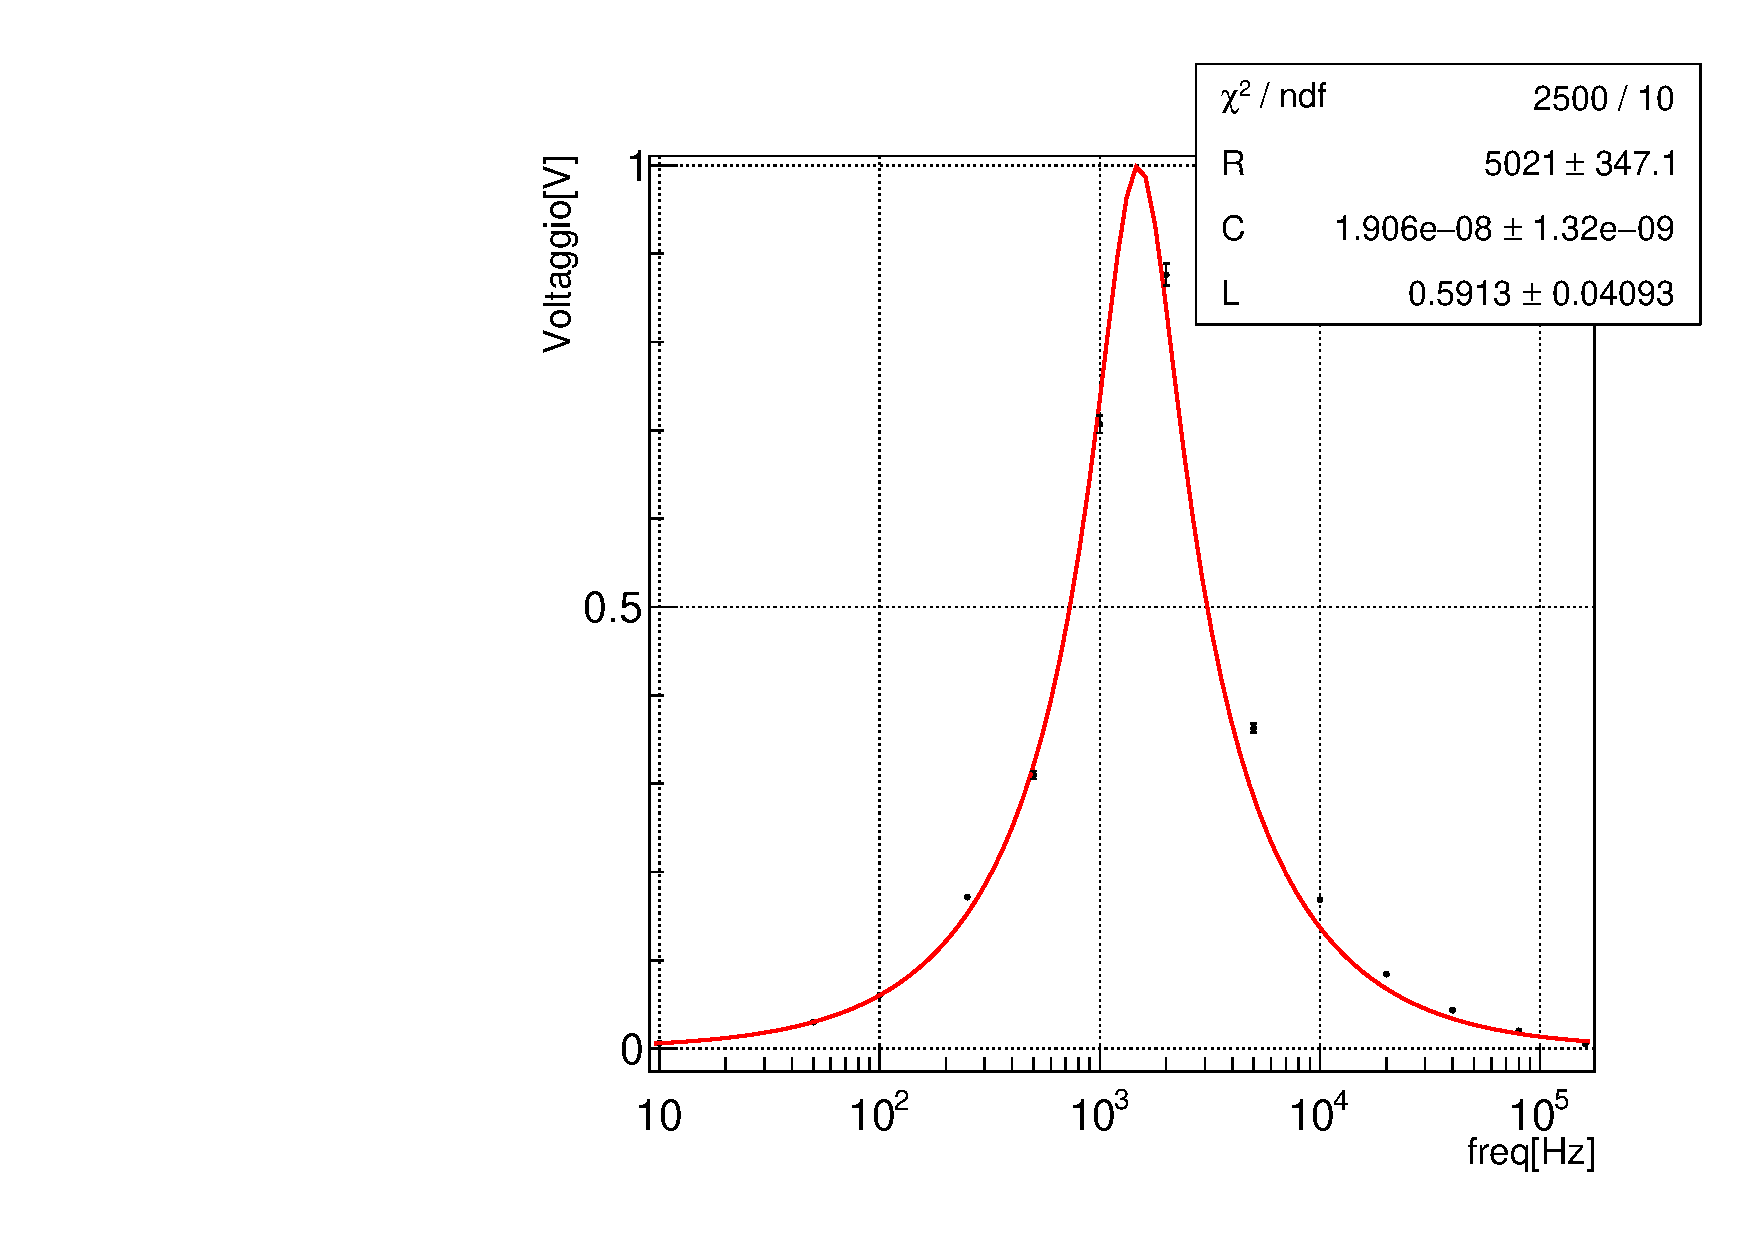
\includegraphics[width=5.7cm]{RLC/RLC-modulo-capoR.pdf}}
\hfill
\subfigure[fase]{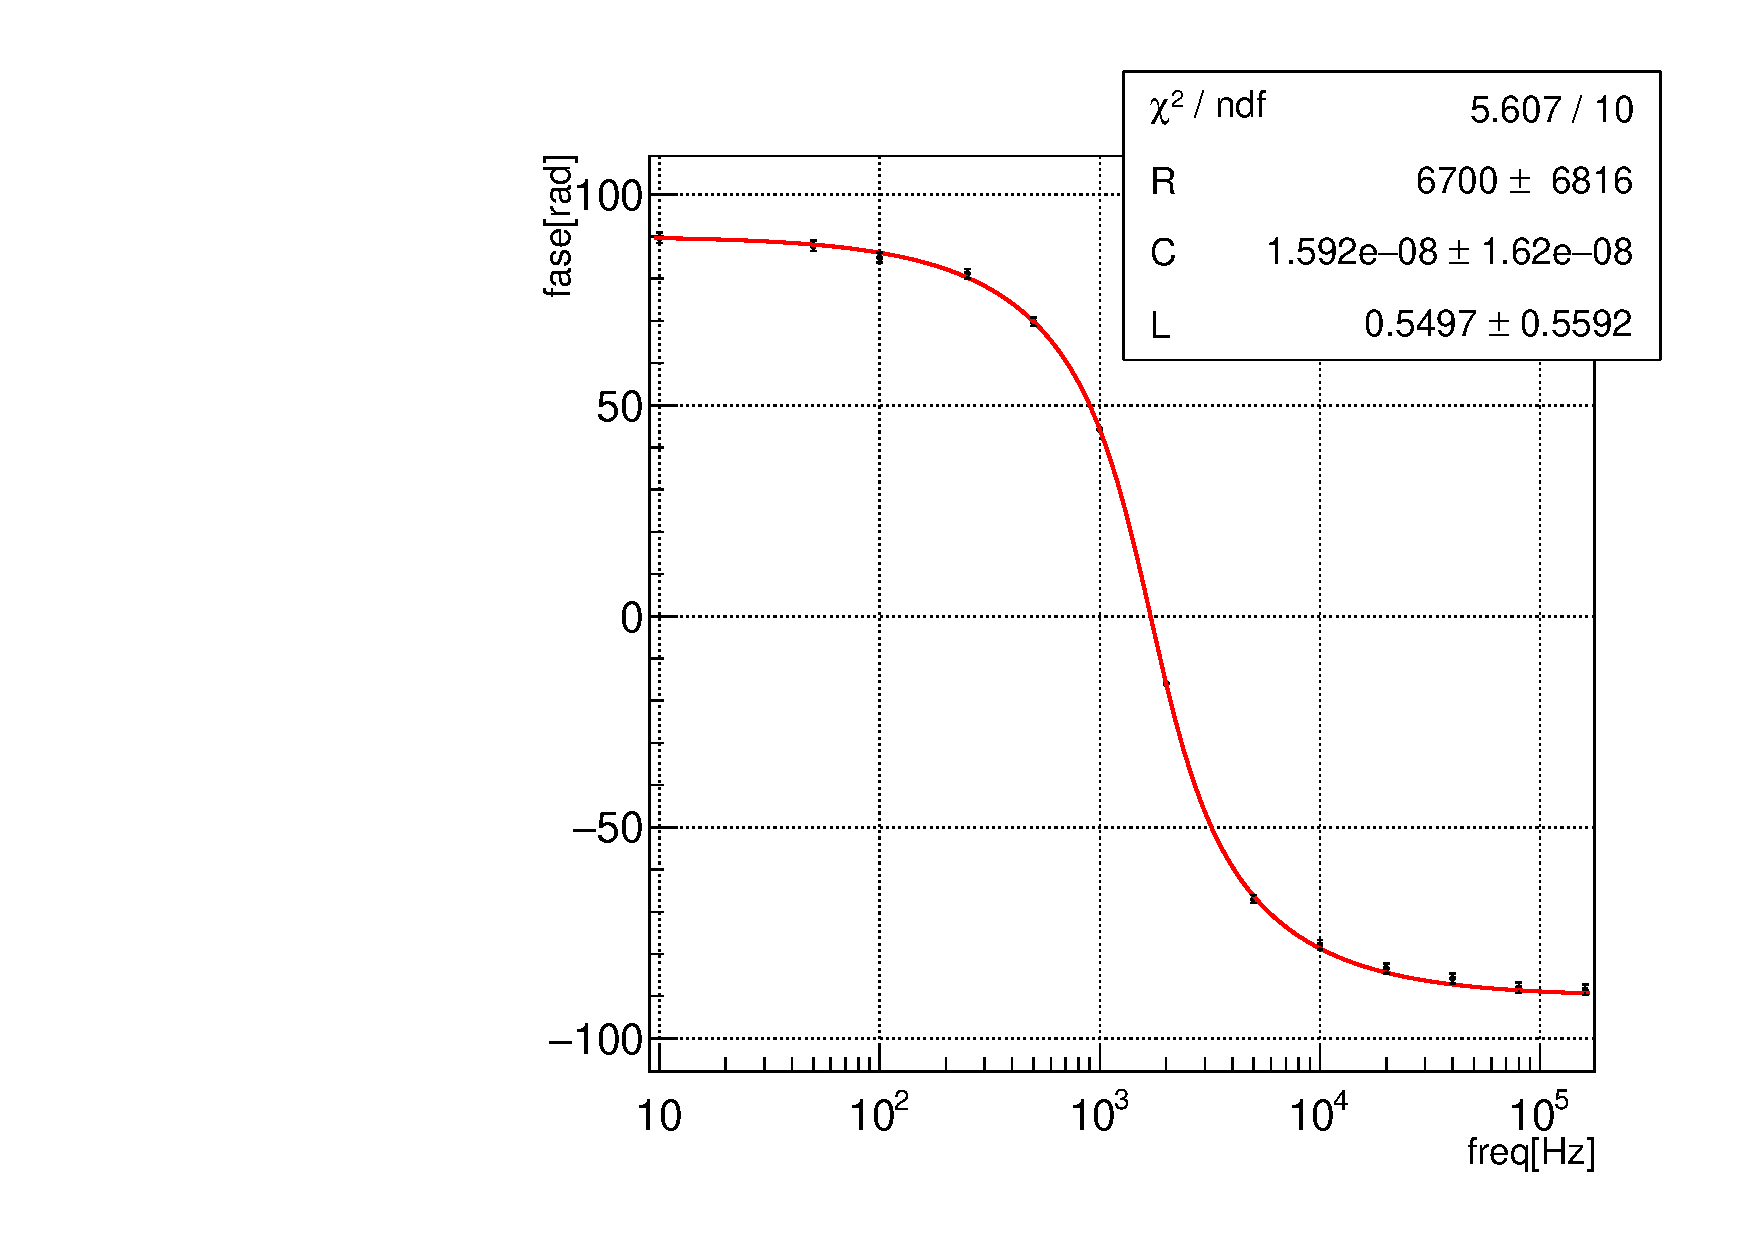
\includegraphics[width=5.7cm]{RLC/RLC-fase-capoR.pdf}}
\hfill
    }
}
\caption*{dal grafico in figura (a) possiamo verificare il ruolo di R nel circuito come filtro passa banda.}
\label{fig:RLC_su_R}
\end{figure}

\noindent Inanzitutto osserviamo che il test del chi quadro sul primo fit non da conclusioni accettabili, infatti risulta \(\chi^{2} = 2500\) mentre Ndf = 10. Questa incongruenza è dovuta ad una anomala disposizione dei punti che pare essere asimmetrica rispetto al picco. Normalmente la funzione di trasferimento ha modulo con andamento a campana la cui larghezza dipende dal valore di R. \\
Supponiamo che, per frequenze alte, il circuito abbia cominicato a comportarsi in maniera inattesa per via dell'attivazione della capacità e dell'induttanza parassite del resistore, le quali hanno aumentato l'entità dell'opposizione di R alla variazione di corrente. Questo fattore di cui R è stato aumentato ha intaccato maggiormente il modulo, ma notiamo che anche la fase dipende da R con andamento \(-arctan\left(\frac{\omega L - \frac{1}{\omega C}}{R}\right)\), quindi per alte frequenze ci aspettiamo di incontrare valori minori in modulo per \(\phi\) di quelli attesi, come infatti è accaduto. \\
\noindent Il test del chi quadro sulla fase riporta un riultato  comunque accettabile perchè grandi variazioni su x si traducono in piccole variazioni su arctan(x); la probabiltà associata al test in questo caso è dell'82\%. \\

\noindent Dalle interpolazioni ricaviamo due stime per R, una data dal modulo, l'altra dalla fase della funzione di trasferimento.
\begin{enumerate}
    \item[-] R dall'interpolazione per il modulo: \(R_{1}=5021 \pm 347 \Omega\)
    \item[-] R dall'interpolazione per la fase: \(R_{2}= 6700 \pm 6816 \Omega\)

\end{enumerate}


\noindent Effettuiamo il test T di Student come segue

\[ t= \frac{\left|R_{1}-R_{2}\right|}{\sqrt{\sigma^2_{R1}+\sigma^2_{R2}}}=0.2\rightarrow PValue = 84.15\% \]\\
 
\noindent Sempre dal grafico ricaviamo il valore di L e di C, utilizzando la stessa formula effettuiamo i dovuti test.

\begin{enumerate}
    \item[-] L dall'interpolazione per il modulo: \(L_{1}= 0.5913 \pm 0.0409 H\)
    \item[-] L dall'interpolazione per la fase:\(L_{2}= 0.5497 \pm 0.5592 H\)

\end{enumerate} 

per cui t = 0.07\(\rightarrow\) PValue =94.42 \%\\

\begin{enumerate}
    \item [-]  C dall'interpolazione per il modulo: \(C_{1}= 1.906\cdot 10^{-8} \pm 1.32\cdot 10^{-9}  F\) 
    \item[-] C dall'interpolazione per la fase: \(C_{2}= 1.592\cdot10^{-8} \pm 1.62\cdot 10^{-8} F \)
\end{enumerate}
 
per cui t = 0.2 \(\rightarrow\) PValue = 84.15\%\\
   
\noindent Osserviamo che le incertezze sulle stime ottenute con la fase sono sempre maggiori in percentuale di quelle ottenute con il modulo. Probabilmente prendendo più punti in prossimità del flesso (dove l'errore sulle fasi intacca poco l'andamento della funzione) avremmo ottenuto maggiore precisione nelle nostre stime. \\
\noindent Effettuiamo infine le medie pesate (pesi = \(w_{i} = \frac{1}{\sigma^{2}_{i}}\)) tra le misure ottenute coi due metodi differenti:\\

\(R_{capoR} = \frac{\sum R_{i}w_{i}}{\sum w_{i}} \pm \frac{1}{\sqrt{\sum w_{i}}}= 5025 \pm 347\Omega\) \\


\(L_{capoR} = \frac{\sum L_{i}w_{i}}{\sum w_{i}} \pm \frac{1}{\sqrt{\sum w_{i}}}= 0.5907 \pm 0.0408 H\) \\

\(C_{capoR} = \frac{\sum C_{i}w_{i}}{\sum w_{i}} \pm \frac{1}{\sqrt{\sum w_{i}}}= (1.904 \pm 0.132) 10^{-8}  F\)\\


\subsubsection{Funzione di trasferimento su C}
Ricaviamo la funzione di trasferimento
\[\vec{V}_{C}(t) = \vec{I}(t)Z_{C} = \frac{\vec{V}_{g}\cdot Z_{C}}{R+j(wL - \frac{1}{wC})}\]
\[\Downarrow\]
\[\vec{H} = \frac{Z_{C}}{R+j(wL - \frac{1}{wC})} \]

\noindent Abbiamo riconosciuto modilo e fase come:

\[\left|\vec{H}\right|=\frac{1}{wC\sqrt{R^2 + (wL - \frac{1}{wC})^2}}\hspace{1cm} (a) \hspace{1cm} \phi_{\vec{H}}= - \frac{\pi}{2} - \arctan\left(\frac{wL- \frac{1}{wC}}{R}\right)\hspace{1cm} (b) \]


\subsubsection*{Dati raccolti}
Questa volta abbiamo visualizzato \(\vec{V}_{in}\) e \(\vec{V}_{out}\) ai capi di C, ottenendo le seguenti misure dalle letture sull'oscilloscopio: 

\begin{table}[!htbp]
\centering
    \captionsetup{labelformat=empty}
    	 \caption{RLC - misure ai capi di C}
    \resizebox{13.5cm}{!}{

    \begin{tabular}{c|c|c|c|c}
        frequenza[Hz] &\(V_{A}\)[V]& \(V_{B}\)[V] & \(V_{B}/V_{A}\) &\(\phi_{B}\)\\
        \hline
        \hline

50   &    20.2 $\pm$ 0.2        & 20.2 $\pm $ 0.2      & 1.00 $\pm$ 0.01 & -2.16 $\pm$ 0.06  \\
\hline
100   &   20.2 $\pm $ 0.2         & 20.2 $\pm $ 0.2  & 1.00 $\pm$ 0.01 & -4.0 $\pm$ 0.1 \\
\hline
250   &   20.2 $\pm $ 0.2         & 20.2 $\pm $ 0.2   & 1.00 $\pm$ 0.01 & -9.7 $\pm$ 0.3 \\
\hline
500  &    20.2 $\pm $ 0.2         & 20.3 $\pm $ 0.2   & 1.00$\pm$ 0.01& -19.4 $\pm$ 0.3 \\
\hline
1000  &   19.8 $\pm $ 0.2         & 20.2 $\pm $ 0.2 & 1.02$\pm$ 0.01 & -45.0 $\pm$ 0.6\\
\hline
1250  &   19.6 $\pm $ 0.2         & 20.1 $\pm $ 0.2  & 1.03 $\pm$ 0.01& -59.4 $\pm$ 0.8 \\
\hline
1500  &   19.2 $\pm $ 0.2         & 17.8 $\pm $ 0.2   & 0.93 $\pm$ 0.01 & -76 $\pm$ 1\\
\hline
2000   &  19.4 $\pm $ 0.2         & 14.4 $\pm $ 0.1  & 0.74 $\pm$ 0.01 & -107 $\pm$ 2\\
\hline
2500  &   19.8 $\pm $ 0.2         & 9.5 $\pm $ 0.1 & 0.481$\pm$ 0.007& -126 $\pm$ 2\\
\hline
3000   &  19.8 $\pm $ 0.2         & 6.84 $ \pm$ 0.07  & 0.345$\pm$ 0.005 & -136 $\pm$ 2 \\
\hline
4000   &  20.0 $ \pm$ 0.2     & 3.84 $ \pm$ 0.04   & 0.192 $\pm$ 0.003& -149 $\pm$ 2  \\
\hline
4500   &  20.2 $ \pm$ 0.2        & 3.04 $\pm $ 0.03 & 0.150 $\pm$ 0.002 & -153 $\pm$ 2\\
\hline
5000  &   20.0 $\pm $ 0.2     & 2.44 $\pm $ 0.02 & 0.122 $\pm$ 0.002& -156 $\pm$ 2\\
\hline
10000  &  20.2 $ \pm$ 0.2         & 0.616 $\pm $ 0.006  & 0.0305 $\pm$ 0.0004 & -169 $\pm$ 2\\
\hline
20000  &  20.2 $ \pm$ 0.2         & 0.152 $\pm $ 0.002    & 0.0075 $\pm$ 0.0001 & -174 $\pm$ 2\\
\hline
40000  &  20.4 $\pm $ 0.2         & 0.04 $\pm $ 0.0004       & 0.00196$\pm$ 0.00003 & -177 $\pm$ 3 \\
        \hline
        \hline
    \end{tabular}
    }
\caption{errore strumentale: 1\%}
\end{table}
        
\subsubsection*{Analisi dati}
Di sotto riportiamo i grafici del caso:


\begin{figure}[!h]
\caption{RCL - funzione di trasferimento ai capi di C}

    \makebox[1 \textwidth][c]{       %centering table
		\resizebox{1.30 \textwidth}{!}{   %resize table
\hfill
\subfigure[modulo]{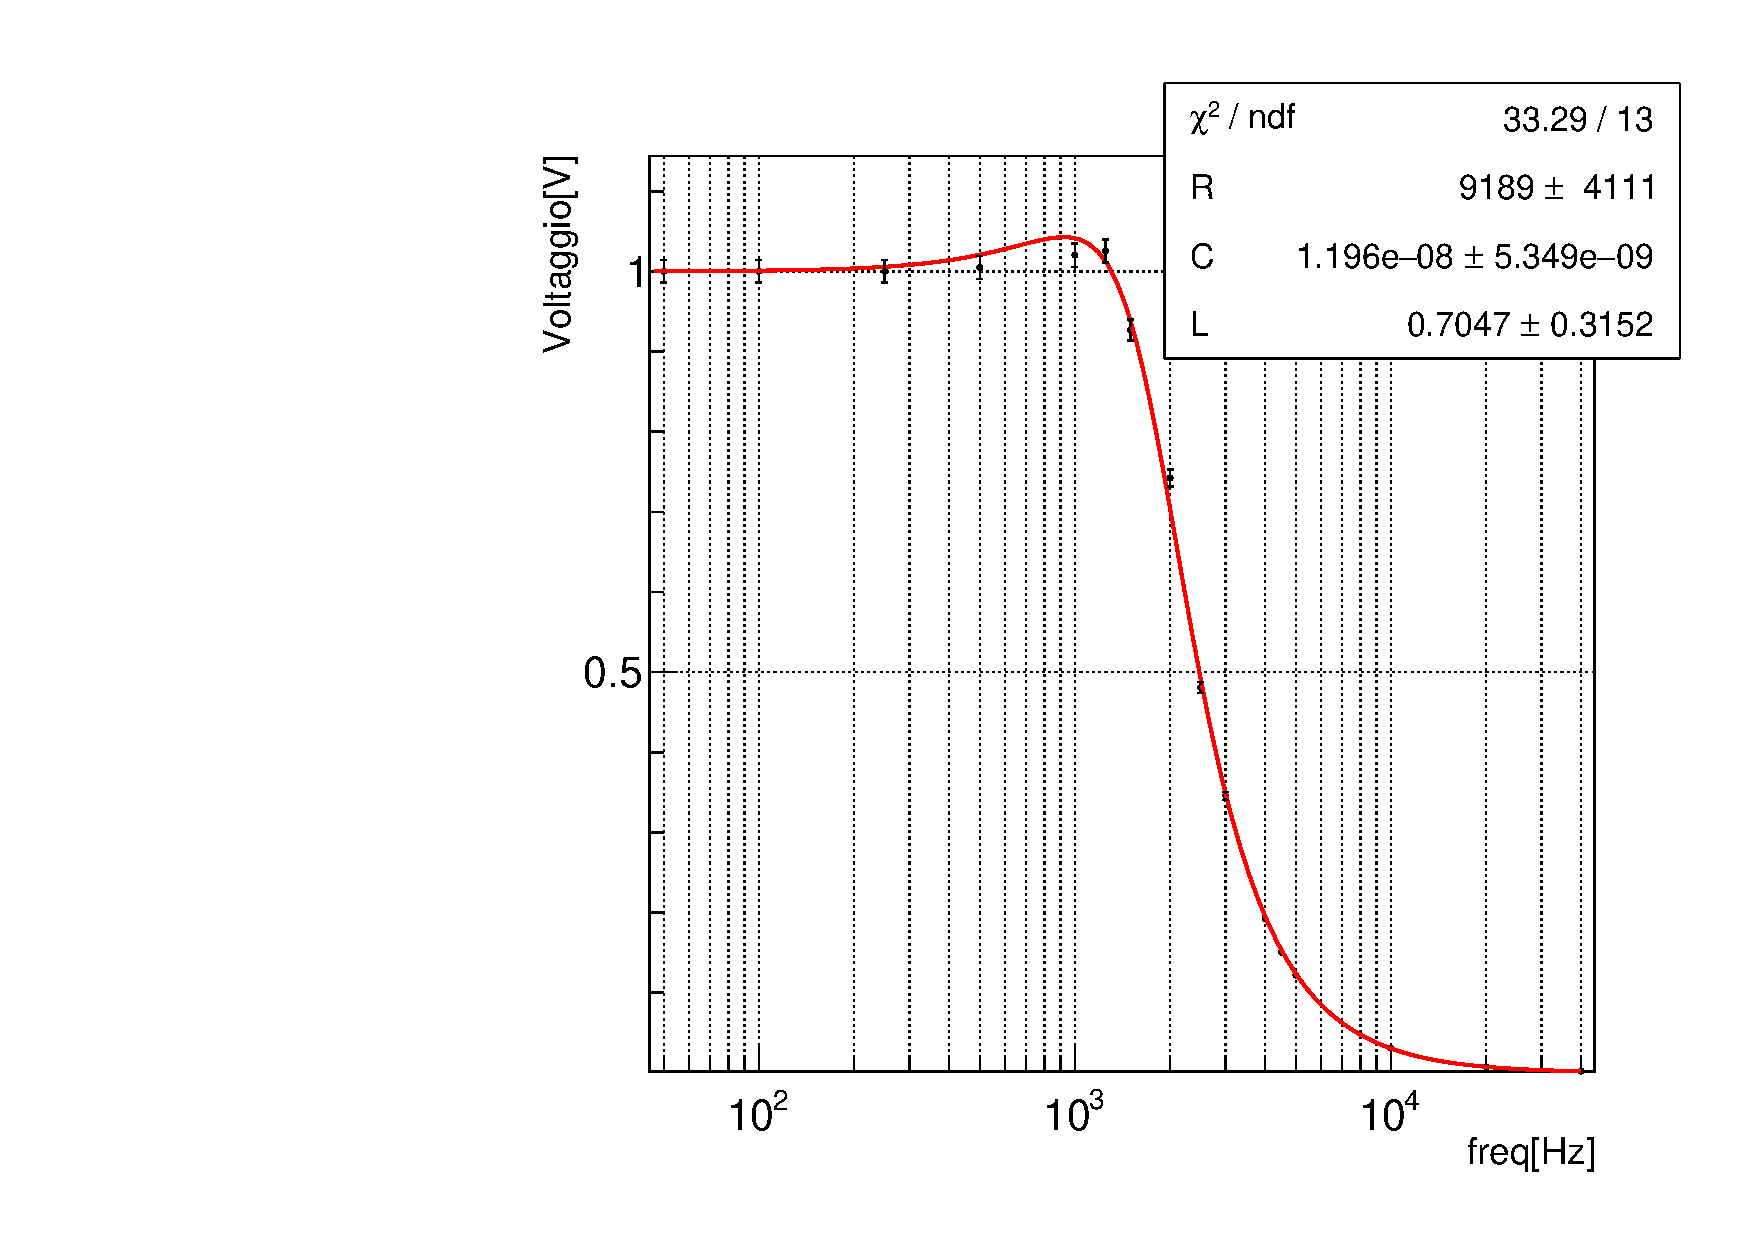
\includegraphics[width=5.7cm]{RLC/RLC-modulo-capoC.pdf}}
\hfill
\subfigure[fase]{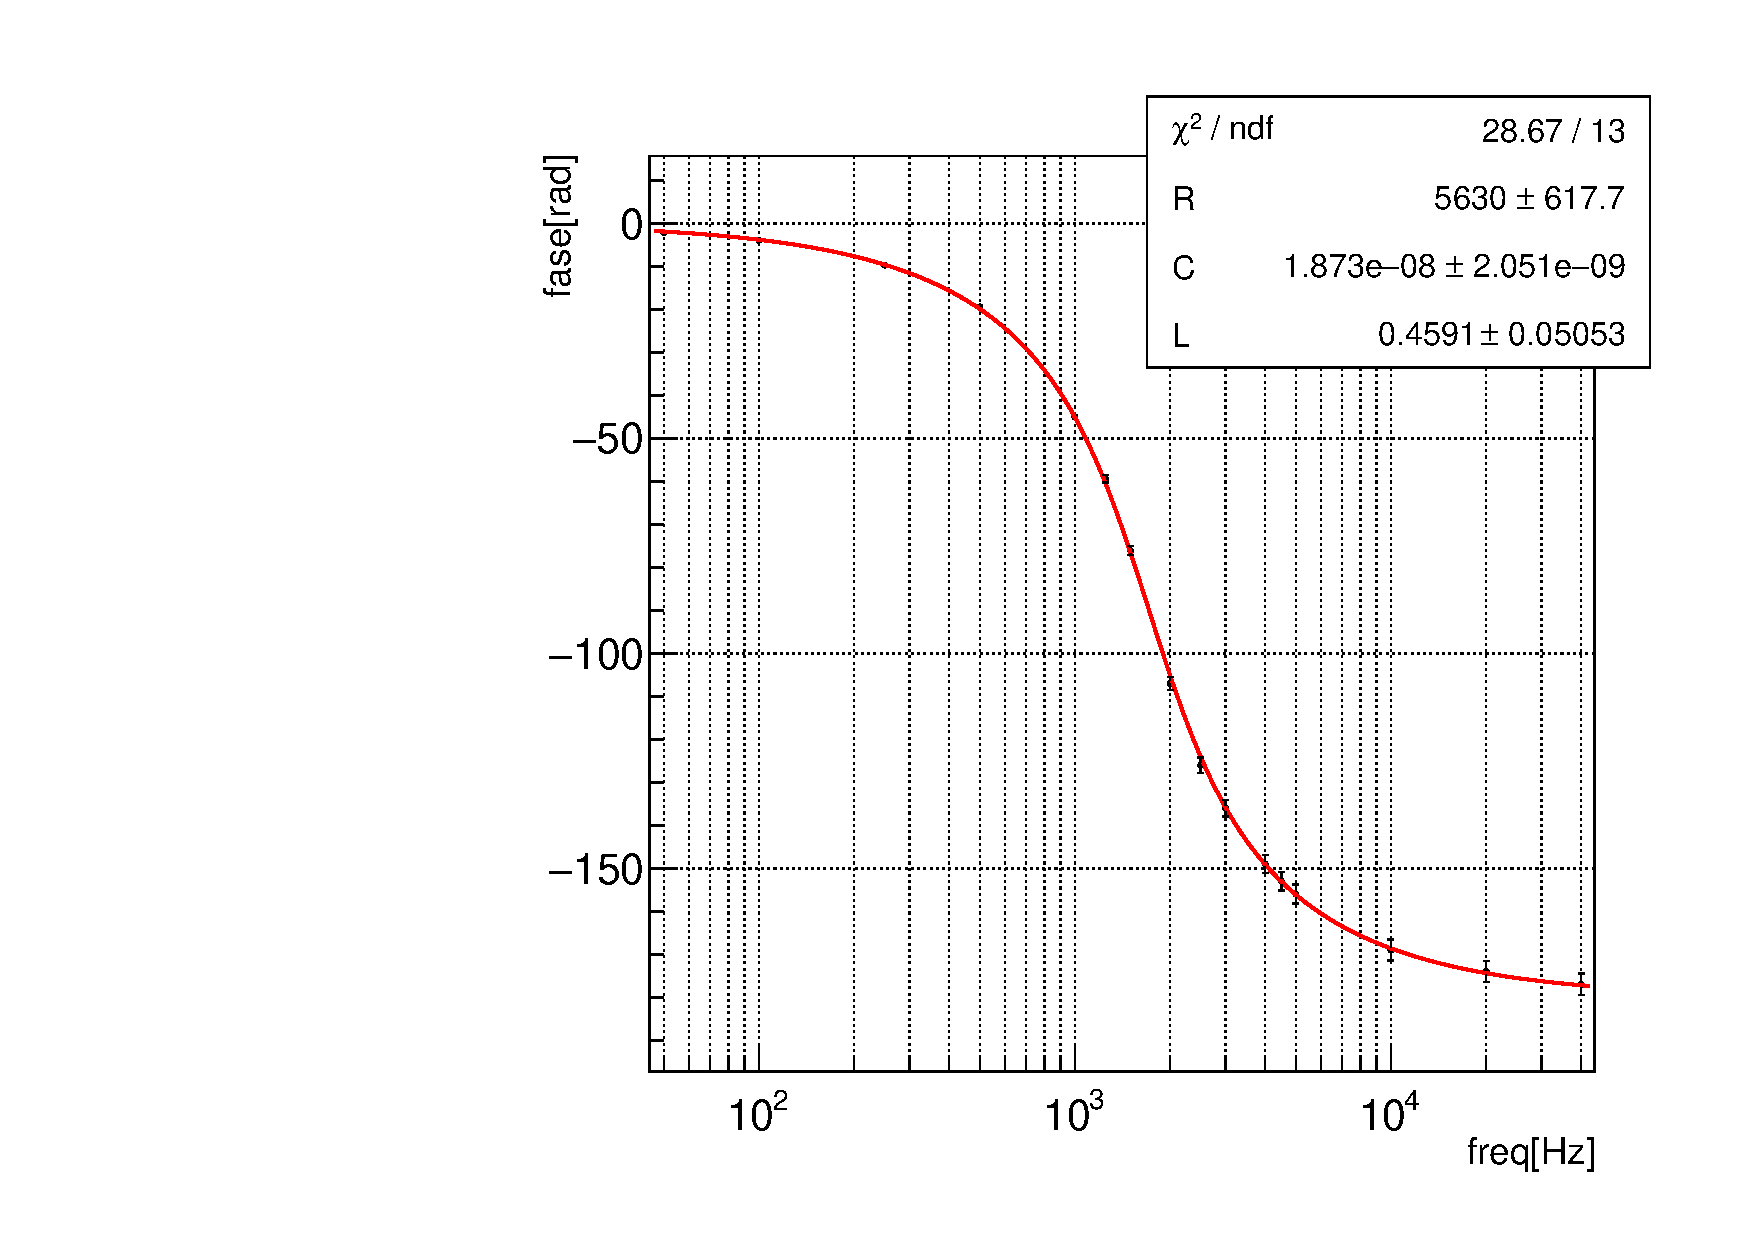
\includegraphics[width=5.7cm]{RLC/RLC-fase-capoC.pdf}}
\hfill
    }
}

\label{fig:RLC_su_C}
\end{figure}

\noindent Il test del chi quadro per il modulo restituisce un \(\chi^{2} = 33.3\) associato al numero di gradi di libertà = 13, che corrisponde ad una probabilità che il nostro modello sia corretto del 0.4\%, accettabile secondo il limite del 0.05\%. Associamo la discrepanza tra \(\chi^{2}\) ed Ndf ad una sottostima degli errori su V, che supponiamo fossero, più realisticamente, maggiori di un fattore \(\sqrt{\frac{\chi^{2}}{Ndf}} = 1.6\). \\
Per quanto riguarda la fase otteniamo \(\chi^{2} = 28.67\) e Ndf = 13, perciò la probabilità risulta del 0.7\% ed il fattore correttivo sulle \(\sigma_{V}\) è  \(\sqrt{\frac{\chi^{2}}{Ndf}} = 1.5\). \\

\noindent Dalle box nei grafici riconosciamo i valori per R, L e C e li analizziamo nel medesimo modus operandi della funzione di trasferimento su R. Per brevità omettiamo il reinserimento delle formule e ci limitiamo a riportare i risultati. \\

\begin{enumerate}
    \item[-] R dall'interpolazione per il modulo: \(R_{1} = 9189 \pm 4111 \Omega\) 
    \item[-]  R dall'interpolazione per la fase:\(R_{2} = 5630 \pm 618 \Omega\)
\end{enumerate} 

da cui t = 0.9\(\rightarrow\) PValue = 36.8 \% \\

\begin{enumerate}
    \item[-] L dall'interpolazione per il modulo: \(L_{1} = 0.7047 \pm 0.3152 H\) 
    \item[-] L dall'interpolazione per la fase: \(L_{2} = 0.4591 \pm 0.0505 H\)
\end{enumerate}
 
dove t = 0.8 \(\rightarrow\) PValue = 36.8\% \\

\begin{enumerate}
    \item[-] C dall'interpolazione per il modulo:\(C_{1} = 1.196 \cdot 10^{-8} \pm 0.535 \cdot 10^{-8} F\)
    \item[-]  C dall'interpolazione per la fase:\(C_{2} = 1.873 \cdot 10^{-8} \pm 0.205 \cdot 10^{-8}\)
 
\end{enumerate}


ca cui t = 1.2 \(\rightarrow\) PValue = 23\% \\

Ora effettuiamo media pesata tra le misure ottenute dai due diversi metodi:\\

\(R_{capoC} = \frac{\sum R_{i}w_{i}}{\sum w_{i}} \pm \frac{1}{\sqrt{\sum w_{i}}}= 5709 \pm 611 \Omega\) \\


\(L_{capoC} = \frac{\sum L_{i}w_{i}}{\sum w_{i}} \pm \frac{1}{\sqrt{\sum w_{i}}}= 0.4652 \pm 0.0499 H\) \\

\(C_{capoC} = \frac{\sum C_{i}w_{i}}{\sum w_{i}} \pm \frac{1}{\sqrt{\sum w_{i}}}= (1.786 \pm 0.191) 10^{-8}  F\)\\

\pagebreak
\subsubsection{Funzione di trasferimento su L}
Scriviamo ancora la legge di Ohm e da qui ricaviamo la funzione di trasferimento su L
\[\vec{V}_{L}(t) = \vec{I}(t)\cdot Z_{L} = \frac{Z_{L}\cdot \vec{V}_{g}}{R + j(wL-\frac{1}{wC})}\]
\[\Downarrow\]
\[\vec{H} = \frac{Z_{L}}{R + j(wL-\frac{1}{wC})}\]
\noindent Identifichiamo modulo e fase con le seguenti formule:

\[\left|\vec{H}\right|= \frac{wL}{\sqrt{R^2+(wL - \frac{1}{wC})^{2}}}\hspace{1cm} (a)\hspace{1cm} \phi_{\vec{H}} = \frac{\pi}{2} - \arctan\left(\frac{wL- \frac{1}{wC}}{R}\right)\hspace{1cm} (b) \]


\subsubsection*{Dati raccolti}
Visualizzando \(\vec{V}_{in}(t)\) e \(\vec{V}_{out}(t)\) ai capi di L siamo riusciti ad ottenere l'ultimo set di dati al variare della frequenza, che riportiamo di sotto: 

\begin{table}[!htbp]
\centering
    \captionsetup{labelformat=empty}
    	 \caption{RCL - misure ai capi di L}
    \resizebox{13.5cm}{!}{

    \begin{tabular}{c|c|c|c|c}
        frequenza[Hz] &\(V_{A}\)[V]& \(V_{B}\)[V] & \(V_{B}/V_{A}\) &\(\phi_{B}\)\\
        \hline
        \hline
        50      & 20.4 $\pm $ 0.2      & 0.0440 $\pm $ 0.0004     & 0.00216 $\pm$ 3\(\cdot 10^{-5}\) & 179 $\pm$ 3\\
        100      &20.4 $\pm $ 0.2         & 0.102 $\pm$ 0.001 & 0.00500 $\pm$ 7 \(\cdot 10^{-5}\)& 176 $\pm$ 2 \\
        250     &20.4 $\pm $ 0.2        & 0.472 $\pm$ 0.005     & 0.0231 $\pm$ 0.0003& 170 $\pm$ 2\\
        500      &20.2 $\pm$ 0.2       & 1.84 $\pm$ 0.02    & 0.091 $\pm$ 0.001& 160 $\pm$ 2 \\
        1000     &19.8 $\pm$ 0.2         & 7.44 $\pm$ 0.07   & 0.376 $\pm$ 0.005  & 135 $\pm$ 2\\
        1250     &19.6 $\pm$ 0.2         & 11.4 $\pm$ 0.1       & 0.582 $\pm$ 0.008& 122 $\pm$ 2 \\
        1500     &19.2 $\pm$ 0.2      & 15.2 $\pm$ 0.2  & 0.79 $\pm$ 0.01& 97 $\pm$ 1 \\
        2000     &19.4 $\pm$ 0.2         & 18.3 $\pm$ 0.2        & 0.94 $\pm$ 0.01& 71 $\pm$ 1\\
        2500     &19.8 $\pm$ 0.2         & 20.5 $\pm$ 0.2        & 1.04 $\pm$ 0.01 & 51.5 $\pm$ 0.7 \\
        3000     &19.8 $\pm$ 0.2         & 20.8 $\pm$ 0.2   & 1.05 $\pm$ 0.01& 39.8 $\pm$ 0.6\\
        4000     &20.0 $\pm$ 0.2             & 20.8 $\pm$ 0.2      & 1.04 $\pm$ 0.01& 28.3 $\pm$ 0.4\\
        4500     &20.2 $\pm$ 0.2        & 20.8 $\pm$ 0.2   & 1.03 $\pm$ 0.01  & 23.5 $\pm$ 0.3\\
        5000     &20.2 $\pm$ 0.2         & 20.6 $\pm$ 0.2    & 1.02 $\pm$ 0.01 & 21.0 $\pm$ 0.3 \\
        10000    &20.2 $\pm$ 0.2         & 20.6 $\pm$ 0.2    & 1.02 $\pm$ 0.01& 10.0 $\pm$ 0.1 \\
        20000    &20.2 $\pm$ 0.2         & 20.4 $\pm$ 0.2     & 1.00 $\pm$ 0.01& 4.7 $\pm$ 0.1 \\
        40000    &20.2 $\pm$ 0.2         & 20.4 $\pm$ 0.2    & 1.01 $\pm$ 0.01& 1.73 $\pm$ 0.05\\
        80000    &20.4 $\pm$ 0.2        & 20.4 $\pm$ 0.2    & 1.00 $\pm$ 0.01  & 1.18 $\pm$ 0.03\\

        \hline
        \hline
    \end{tabular}
    }
\caption{errore strumentale: 1\%}
\end{table}
\subsubsection*{Analisi dati}
La funzione di trasferimento ai capi di L presentava gli andamenti riportati nei seguenti grafici:

\begin{figure}[!h]
\caption{RCL - funzione di trasferimento ai capi di L}

    \makebox[1 \textwidth][c]{       %centering table
		\resizebox{1.30 \textwidth}{!}{   %resize table
\hfill
\subfigure[modulo]{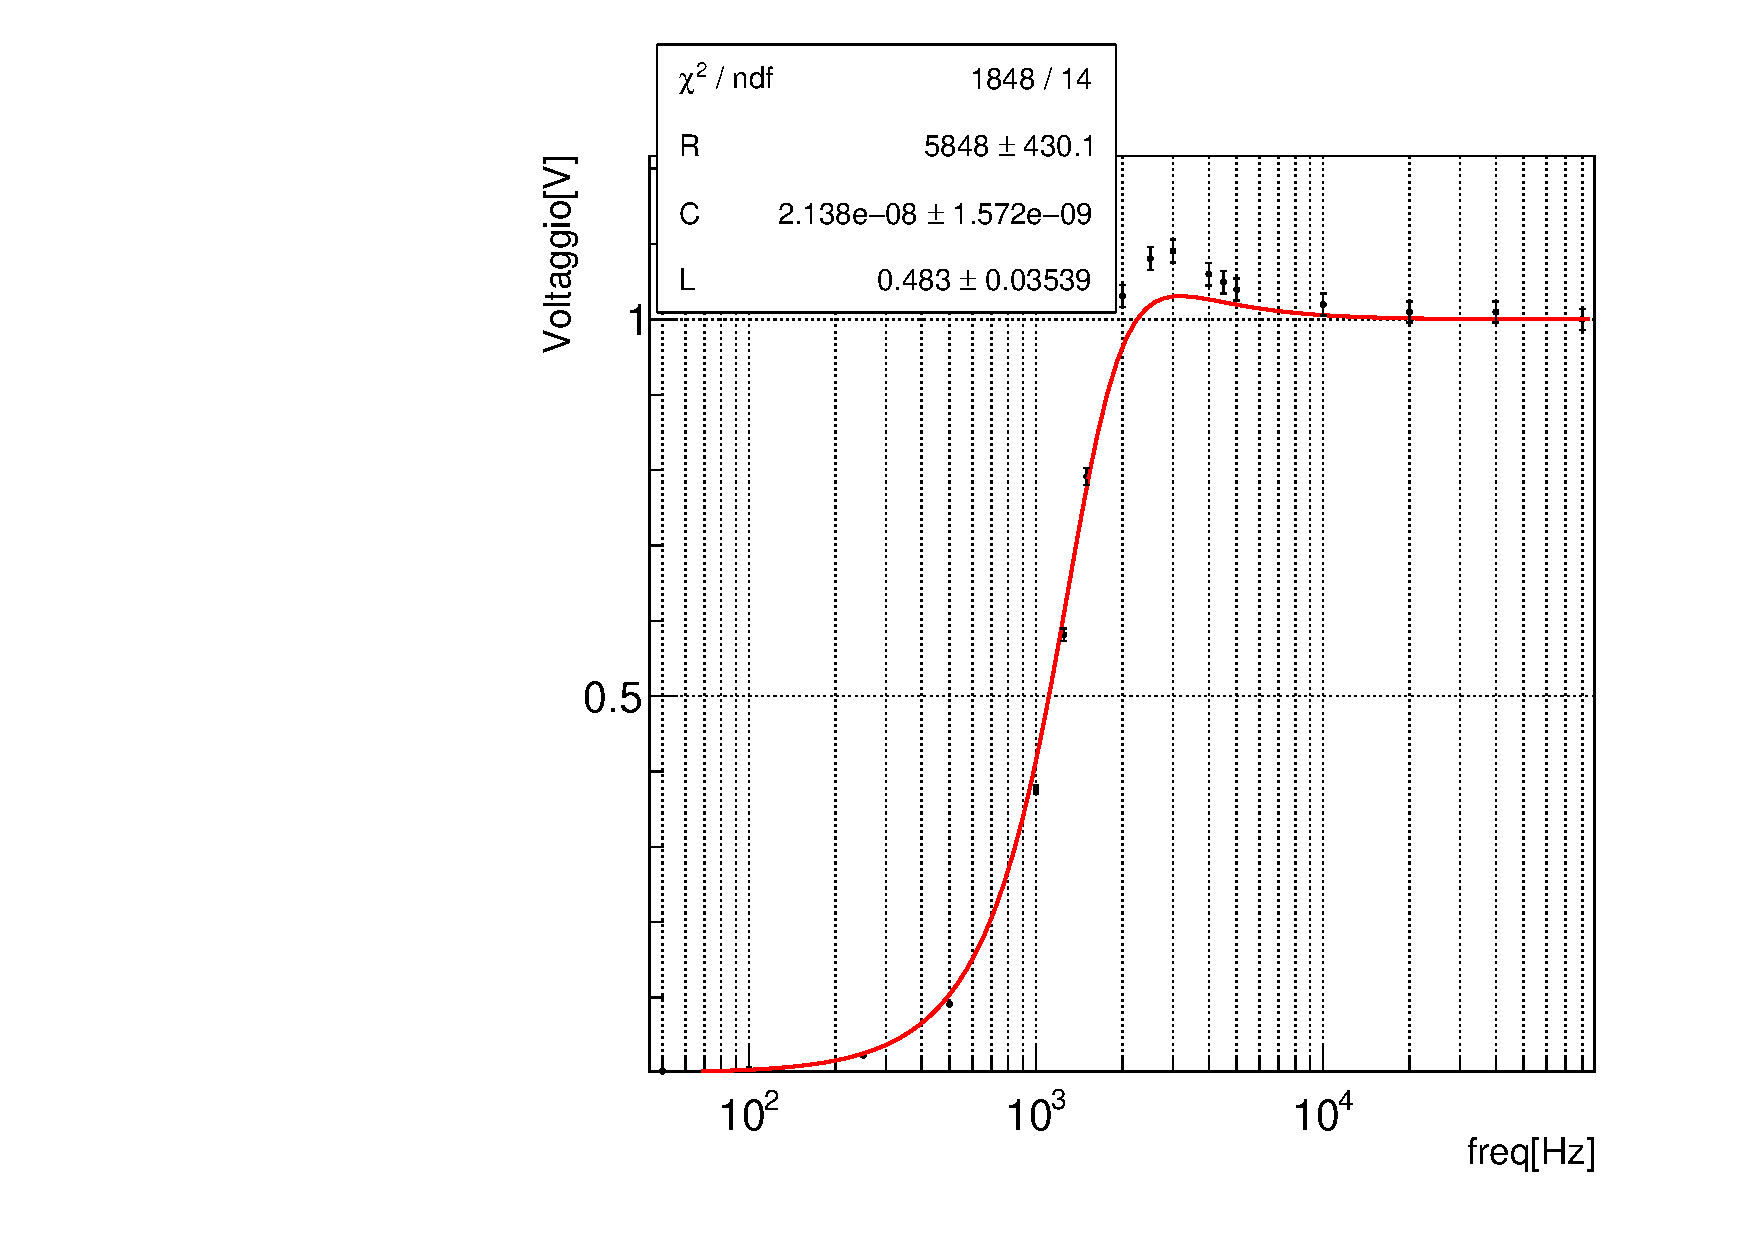
\includegraphics[width=5.7cm]{RLC/RLC-modulo-capoL.pdf}}
\hfill
\subfigure[fase]{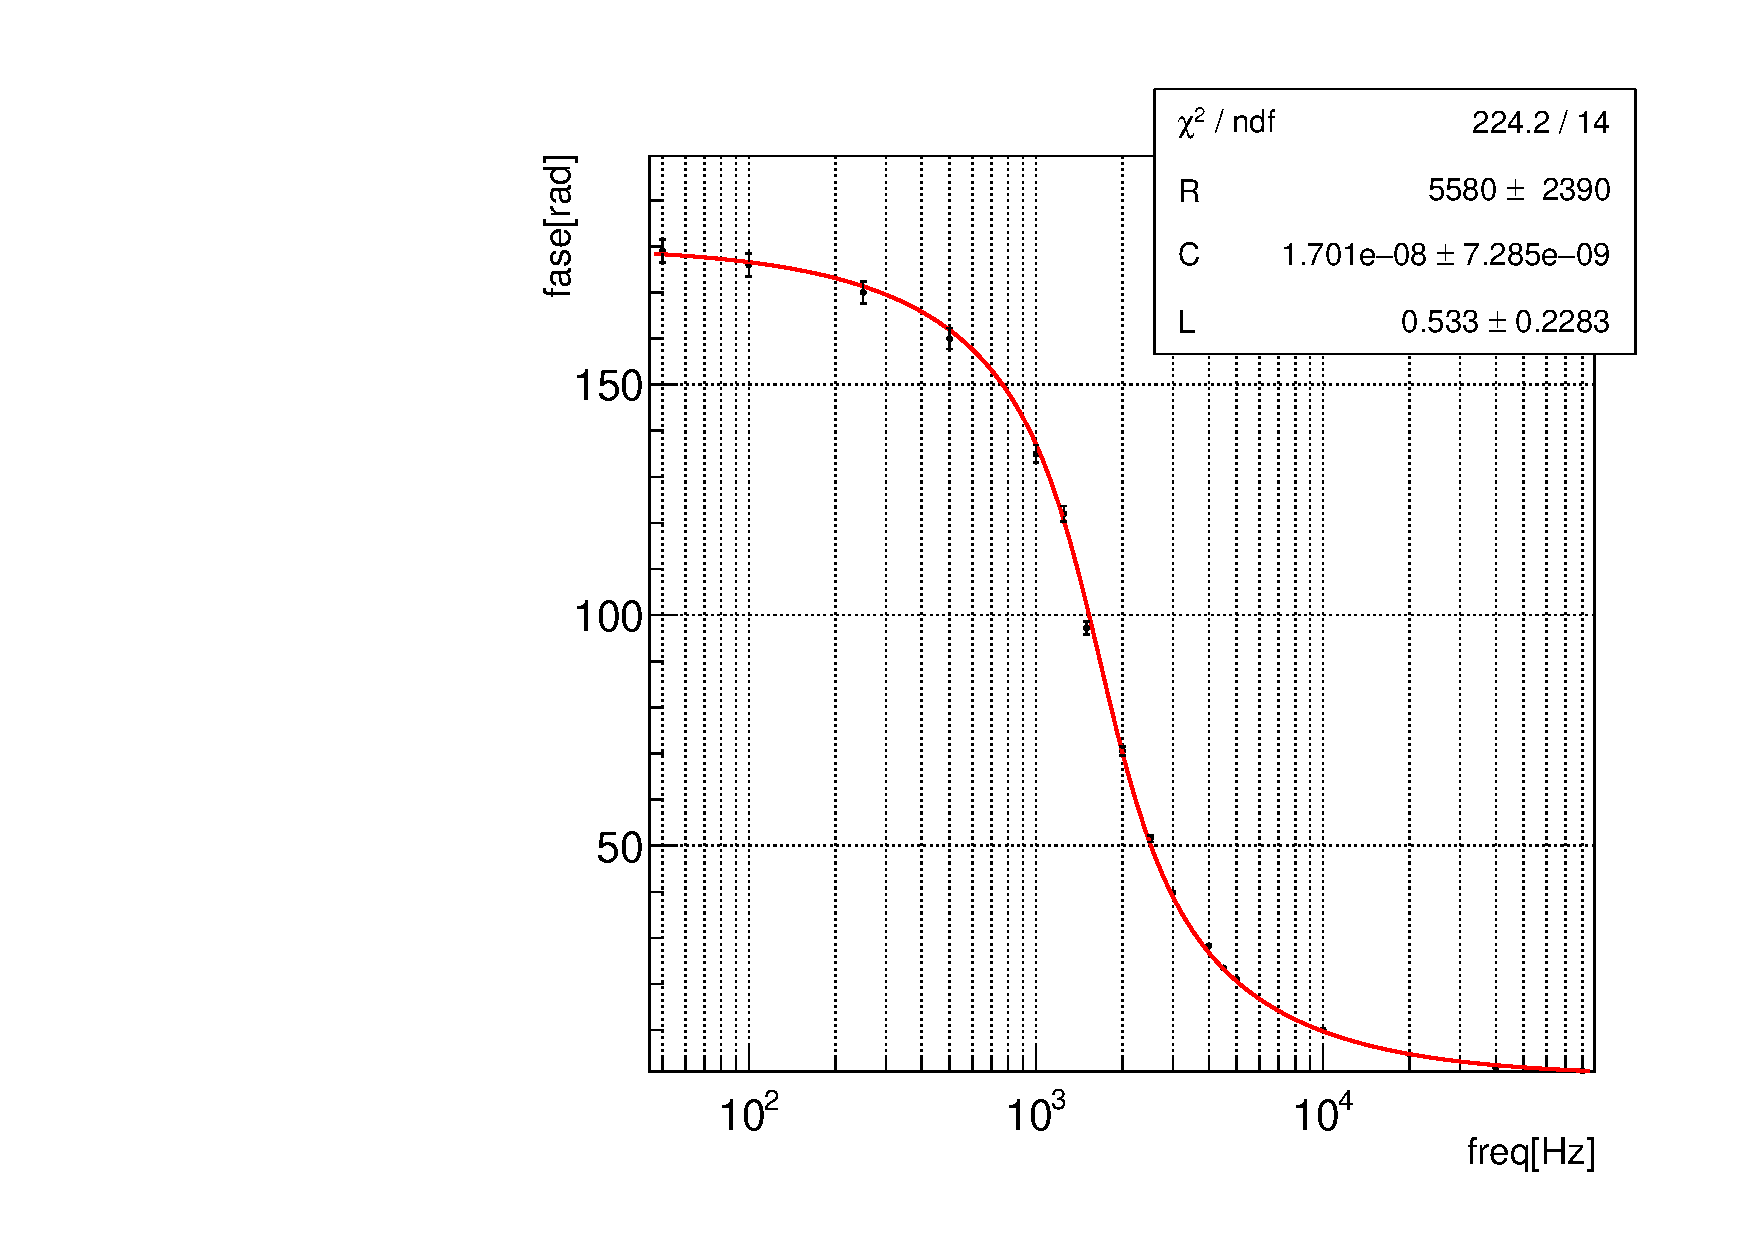
\includegraphics[width=5.7cm]{RLC/RLC-fase-capoL.pdf}}
\hfill
    }
}

\label{fig:RLC_su_L}
\end{figure}

\noindent Entrambi i test effettuati con ROOT non restituiscono risultati accettabili, è possibile che i modelli adoperati per l'interpolazione non fossero sufficientemente compatibili con la realtà. Avanziamo l'ipotesi che scegliendo una resistenza maggiore, tale da contrastare il valore della resistenza interna dell'induttanza il quale, variando con la frequenza, tende a causare anomalie nel circuito, avremmo ottenuto un comportamento più prevedibile. \\

\noindent Riportiamo le stime ottenute per i parametri del circuito: 
\begin{enumerate}
    \item [-] R dall'interpolazione per il modulo: \(R_{1} = 5848 \pm 430 \Omega\) 
    \item[-] R dall'interpolazione per la fase:\(R_{2} = 5580\pm 2390 \Omega\) 
\end{enumerate}

da cui t = 0.1 \(\rightarrow\) PValue = 92 \% \\

\begin{enumerate}
    \item[-] L dall'interpolazione per il modulo: \(L_{1} = 0.483 \pm 0.035  H\)
    \item[-]L dall'interpolazione per la fase: \(L_{2} = 0.533 \pm 0.228 H\)
\end{enumerate}
 
abbiamo ottenuto t = 0.2 \(\rightarrow\) PValue = 84\% \\

\begin{enumerate}
    \item[-] C dall'interpolazione per il modulo:\(C_{1} = 2.138\cdot 10^{-8} \pm 0.157\cdot 10^{-8} F\)
    \item[-] C dall'interpolazione per la fase:\(C_{2} = 1.701 \cdot 10^{-8} \pm 0.729 \cdot 10^{-8}\) 
\end{enumerate}


con t = 0.6 \(\rightarrow\) PValue = 54.85 \%\\

\noindent Abbiamo effettuato la media pesata tra le misure ottenute dai due diversi metodi:


\(R_{capoL} = \frac{\sum R_{i}w_{i}}{\sum w_{i}} \pm \frac{1}{\sqrt{\sum w_{i}}} = 5840 \pm 423 \Omega\) \\


\(L_{capoL} = \frac{\sum L_{i}w_{i}}{\sum w_{i}} \pm \frac{1}{\sqrt{\sum w_{i}}}= 0.4842 \pm 0.0346 H\) \\

\(C_{capoL} = \frac{\sum C_{i}w_{i}}{\sum w_{i}} \pm \frac{1}{\sqrt{\sum w_{i}}}= (2.119 \pm 0.153) 10^{-8}  F\)\\

\pagebreak
\subsubsection{Conclusioni circuiti LCR - RLC - RCL}
Una grandezza significativa per questo tipo di circuiti è la frequenza di risonanza. In corrispondenza di \(f = \frac{1}{2\pi \sqrt{LC}}\) si ha generalmente il picco per \(\left| \vec{H}\right|\), andiamo a calcolare la frequenza di risonanza utilizzando le migliori stime dei i parametri del circuito ottenute per ogni caso. \\
\begin{enumerate}
    \item[-] ai capi di R, \(f = \frac{1}{2\pi \sqrt{L_{capoR} C_{capoR}}} = 1500  \pm 55 Hz\)
    
    \item[-] ai capi di C, \(f = \frac{1}{2\pi \sqrt{L_{capoC} C_{capoC}}} = 1746  \pm 132 Hz\)
    
    \item[-] ai capi di L, \(f = \frac{1}{2\pi \sqrt{L_{capoL} C_{capoL}}} = 1571 \pm 80 Hz\)
\end{enumerate}

\noindent Concludiamo confrontando fra loro le stime ottenute per R, L e C in questa seconda parte. \\

\noindent Considerando una probabilità limite del 0.05\%: 

\begin{enumerate}
    \item resistore:
    \begin{enumerate}
        \item \(R_{capoR} = 5025 \pm 347 \Omega\)
        \item \(R_{capoC} = 5709 \pm 611 \Omega \Rightarrow\) sono tutti compatibili,\(\bar{R} = 5410 \pm 246 \Omega\)
        \item \(R_{capoL} = 5840 \pm 423 \Omega\)
    \end{enumerate}
    \item capacitore:
    \begin{enumerate}
        \item \(C_{capoR} = 19.04 \pm 1.32  nF\)
        \item \(C_{capoC} = 17.86 \pm 1.91 nF \Rightarrow\) sono tutti compatibili,\(\bar{C} = 19.5 \pm 0.9\)nF
        \item \(C_{capoL} = 21.19 \pm 1.53 nF\)
    \end{enumerate}
    \item induttanza:
    \begin{enumerate}
        \item \(L_{capoR} = 0.5907 \pm 0.0408 H\)
        \item \(L_{capoC} = 0.4652 \pm 0.0499H \Rightarrow\) sono tutti compatibili,\(\bar{L} = 0.54  \pm 0.02 \)H
        \item \(L_{capoL} = 0.4842 \pm 0.0346 H\)
    \end{enumerate}
\end{enumerate}
   




\end{document}
